\documentclass[11pt,letterpaper]{article}
\usepackage[margin=0.8in,headheight=15pt]{geometry}
\usepackage{fontspec}
\setmainfont{texgyrepagella}[Extension=.otf,UprightFont=*-regular,BoldFont=*-bold,ItalicFont=*-italic,BoldItalicFont=*-bolditalic]
\setsansfont{texgyreheros}[Extension=.otf,UprightFont=*-regular,BoldFont=*-bold,ItalicFont=*-italic,BoldItalicFont=*-bolditalic]
\usepackage{amsmath,amssymb,booktabs,tabularx,array,enumitem,xcolor}
\usepackage{tikz}
\usetikzlibrary{arrows.meta,positioning,calc}
\usepackage{fancyhdr,hyperref}
\definecolor{forest}{HTML}{24594B}
\definecolor{pale}{HTML}{EFF5F1}
\definecolor{blue}{HTML}{305F82}
\definecolor{orange}{HTML}{9C5424}
\hypersetup{colorlinks=true,linkcolor=forest,urlcolor=blue,pdftitle={Shawn's Ecology Study Book 1A to 2C},pdfauthor={Prepared for Shawn}}
\pagestyle{fancy}\fancyhf{}
\fancyhead[L]{\small\sffamily SHAWN'S BIOLOGY}
\fancyhead[R]{\small\sffamily ECOLOGY\quad 1A--2C}
\fancyfoot[C]{\small\thepage}
\renewcommand{\headrulewidth}{0pt}
\setlength{\emergencystretch}{1em}
\setlength{\parindent}{0pt}\setlength{\parskip}{6pt}
\setlist[itemize]{leftmargin=1.3em,itemsep=3pt,topsep=3pt}
\setlist[enumerate]{leftmargin=1.6em,itemsep=6pt,topsep=3pt}
\renewcommand{\arraystretch}{1.24}
\newcolumntype{Y}{>{\raggedright\arraybackslash}X}
\newcommand{\pagechapter}[2]{\clearpage\section*{#1}\phantomsection\label{#2}\addcontentsline{toc}{section}{#1}}
\newcommand{\idea}[1]{\textbf{Main idea.} #1\par}
\newcommand{\term}[2]{\textbf{#1}: #2}
\newcommand{\memorycheck}[1]{\par\smallskip\textbf{Try from memory.} #1\par}
\newcommand{\source}[1]{{\footnotesize\textit{Further reading:} #1\par}}
\tikzset{concept/.style={draw=forest,fill=pale,rounded corners=3pt,align=center,font=\small\sffamily,text width=3.4cm,minimum height=1cm,inner sep=6pt}, flow/.style={-{Stealth[length=2.5mm]},thick,draw=forest}, rel/.style={font=\scriptsize\sffamily,fill=white,inner sep=2pt,align=center,text=black}}
\newcommand{\classsource}[1]{{\footnotesize\textit{Class connection:} #1\par}}
\makeatletter
\renewcommand{\l@section}{\@dottedtocline{1}{0em}{0em}}
\makeatother
\pdfstringdefDisableCommands{\def\quad{ }}
\begin{document}
\hypersetup{pageanchor=false}
\begin{titlepage}
\vspace*{0.7in}
{\sffamily\large BIOLOGY STUDY COLLECTION\par}
\vspace{0.35in}
{\Huge\bfseries Ecology\par}
\vspace{0.15in}
{\LARGE Knowledge and connections\par}
\vspace{0.25in}
{\Large Learning targets 1A through 2C\par}
\vspace{0.3in}
{\large Prepared for Shawn\par}
\vspace{0.5in}

\begin{tikzpicture}
\node[concept] (a) at (0,0) {Evidence};
\node[concept] (b) at (5.2,0) {Living systems};
\node[concept] (c) at (10.4,0) {Ecological change};
\draw[flow] (a)--node[rel,above]{explains}(b);
\draw[flow] (b)--node[rel,above]{respond to}(c);
\end{tikzpicture}\par
\vspace{0.45in}
This book connects scientific reasoning, homeostasis, energy and matter, biodiversity, and population ecology. Use the diagrams to explain relationships, then test your understanding with the questions at the end.

\textbf{Scope.} The teacher's \textit{Ecology Unit Guide} sets the learning targets. Shawn has covered 1A--2C. The supplied StudyBio practice quiz informs the review emphasis; it is not confirmation of the next exam's scope.

\textbf{How to use the book.} Read one section, close the book, and explain its main idea aloud. Redraw the related graph with labeled arrows. Attempt the review questions before checking the answers.
\vfill
{\small Original study explanations and diagrams supplement the teacher's outline. Class-specific policies and grading requirements must come from the class materials. Source notes and practice-key clarifications appear at the end.\par}
\end{titlepage}
\hypersetup{pageanchor=true}
{\setlength{\parskip}{0pt}\small\tableofcontents}
\vspace{12pt}
\textbf{Review sequence.} Start with 1A and 1B, then connect metabolism to ecosystems in 1C. Use those ideas to explain biodiversity in 2A, human impacts in 2B, and population change in 2C.

\textbf{A useful answer has three parts:} name the concept, describe the mechanism, and apply the mechanism to the particular organism, ecosystem, or data.

\pagechapter{The knowledge graph}{graph}
\idea{Ecology connects mechanisms at different scales. Read each arrow as a sentence, not just a line between words.}
\begin{center}
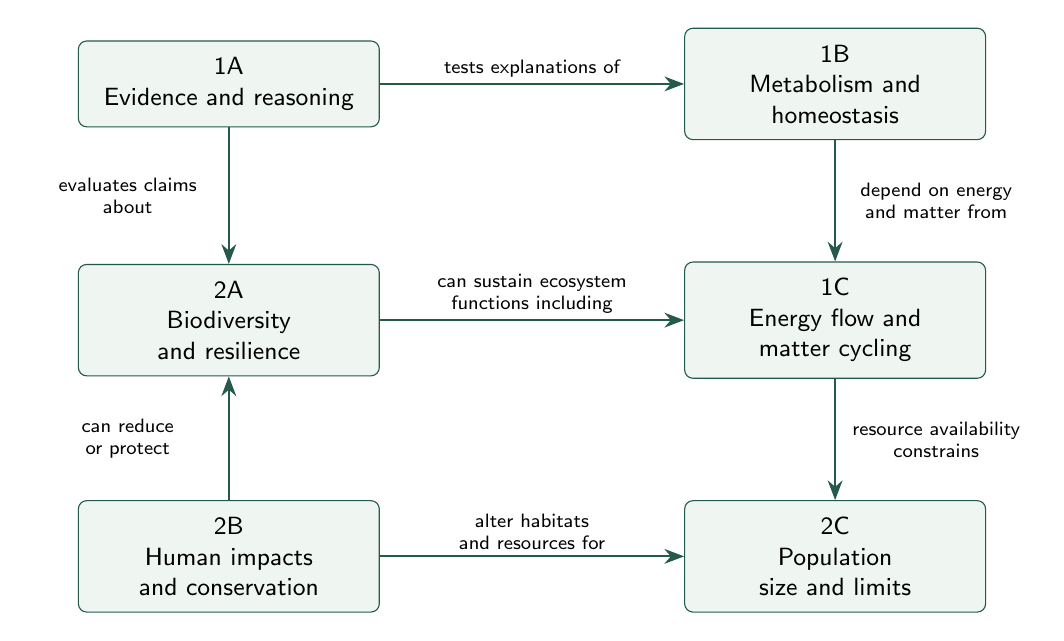
\begin{tikzpicture}[x=1cm,y=1cm]
\node[concept] (a) at (0,0) {1A\\Evidence and reasoning};
\node[concept] (b) at (7.7,0) {1B\\Metabolism and homeostasis};
\node[concept] (c) at (7.7,-3) {1C\\Energy flow and matter cycling};
\node[concept] (d) at (0,-3) {2A\\Biodiversity and resilience};
\node[concept] (e) at (0,-6) {2B\\Human impacts and conservation};
\node[concept] (f) at (7.7,-6) {2C\\Population size and limits};
\draw[flow] (a)--node[rel,above]{tests explanations of}(b);
\draw[flow] (b)--node[rel,right,text width=2.4cm]{depend on energy\\and matter from}(c);
\draw[flow] (d)--node[rel,above]{can sustain ecosystem\\functions including}(c);
\draw[flow] (e)--node[rel,left,text width=2.4cm]{can reduce\\or protect}(d);
\draw[flow] (c)--node[rel,right,text width=2.4cm]{resource availability\\constrains}(f);
\draw[flow] (e)--node[rel,above]{alter habitats\\and resources for}(f);
\draw[flow] (a)--node[rel,left,text width=2.4cm]{evaluates claims\\about}(d);
\end{tikzpicture}\par
\end{center}
\subsection*{Three connections to explain}
\begin{enumerate}
\item \textbf{Organism to ecosystem:} cellular respiration supplies usable energy for homeostasis; food webs trace where the energy in an organism's food came from.
\item \textbf{Habitat to population:} habitat loss can reduce food and nesting sites, lowering carrying capacity and changing births, deaths, and movement.
\item \textbf{Biodiversity to resilience:} species that respond differently to disturbance can help ecosystem functions continue when one species declines.
\end{enumerate}
\memorycheck{Explain a path from human habitat change to a change in biodiversity, then to an ecosystem service people use.}

\pagechapter{1A\quad Evidence and scientific reasoning}{onea}
\idea{Science builds explanations from observations, tests predictions, and revises explanations when evidence changes. Deliberate practice improves how clearly you do this.}
\subsection*{Distinctions to know}
\par
\begin{tabularx}{\linewidth}{@{}p{0.26\linewidth}Y@{}}\toprule
Concept & Meaning and example\\\midrule
Observation & What is measured or detected: ``The plant is 12 cm tall.''\\
Inference & An interpretation: ``The plant may be growing slowly because it receives little light.''\\
Quantitative data & Numerical measurements or counts, such as 12 cm or 8 seedlings.\\
Qualitative data & Descriptions, such as yellow leaves or cloudy water.\\
Induction & Particular observations lead to a broader explanation; repeated observations of shaded plants suggest a light--growth relationship.\\
Deduction & A general idea leads to a specific prediction: if light limits growth, otherwise similar plants given more light should grow more.\\\bottomrule
\end{tabularx}
\par
\subsection*{How the reasoning fits together}
An observation suggests a question. A testable explanation leads to a prediction. Measurements are compared with the prediction. Results can support an explanation, expose a weakness, or suggest a new question. One favorable result does not prove that an explanation is always true.

\textbf{Example.} A plant near a window is taller than a plant in a cupboard. The height difference is an observation. A claim that light caused the difference is an inference; water, species, and starting size could also differ.
\subsection*{Learning vocabulary}
\term{Annotation}{a note that identifies a key idea, question, or connection.}
\term{Formative assessment}{a check used to guide learning and feedback.}
\term{Summative assessment}{a check of achievement after a period of learning.}

Use \textbf{feedback} to identify a specific gap, practice the missing skill, and reassess. \textbf{Collaboration} includes comparing reasoning and explaining ideas; individual understanding still needs to be demonstrated.

\textbf{Class-specific information.} See page \pageref{classroom} for the supplied class expectations and grading overview.
\memorycheck{Change ``The pond is unhealthy'' into one measurable observation and one clearly labeled inference.}

\pagechapter{1A\quad Class expectations and scientific investigation}{classroom}
\idea{Use the learning targets to guide practice and the evidence to guide your conclusions.}
\subsection*{The assessment system in the class slides}
KUDOS provides the broad overview. The unit guide lists detailed vocabulary and study questions. Classwork, homework, notes, and review prepare students for the unit exams.
\par
\begin{tabularx}{\linewidth}{@{}p{0.26\linewidth}Y@{}}\toprule
Assessment & Supplied class policy\\\midrule
Formative practice & Homework, practice tests, and CFAs give feedback without directly affecting grades.\\
Checkups & 15\% of the grade; cover assigned work. Lowest two per semester dropped. No retake or makeup except for an excused absence.\\
Quality assignments & 20\% of the grade.\\
Quizzes and exams & 45\%. The unit exam can replace the quiz score. Exam retakes are available for scores below 80\%, with homework completion and a retake ticket required.\\
Final exam & 20\% of the grade.\\\bottomrule
\end{tabularx}\par
The slides estimate 15--30 minutes of focused homework nightly. If a student still struggles after more than an hour of focused work, they advise contacting the teacher and seeking tutorial help. These summarize the supplied deck; later teacher announcements may update policies.
\subsection*{Observations become testable explanations}
\begin{center}
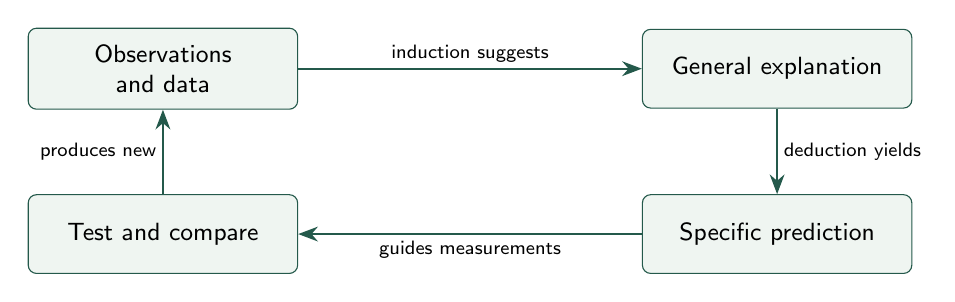
\begin{tikzpicture}[concept/.append style={text width=3cm}]
\node[concept] (o) at (0,0) {Observations and data};
\node[concept] (e) at (7.8,0) {General explanation};
\node[concept] (p) at (7.8,-2.1) {Specific prediction};
\node[concept] (t) at (0,-2.1) {Test and compare};
\draw[flow] (o)--node[rel,above]{induction suggests}(e);
\draw[flow] (e)--node[rel,right]{deduction yields}(p);
\draw[flow] (p)--node[rel,below]{guides measurements}(t);
\draw[flow] (t)--node[rel,left]{produces new}(o);
\end{tikzpicture}\par
\end{center}
A \textbf{hypothesis} is a testable proposed explanation. A \textbf{prediction} states a result expected if that explanation applies. Deduction guarantees a conclusion only with a valid argument and true premises; inductive conclusions remain revisable. Science uses both forms.
\textbf{Geotastic example.} A visible road sign is an observation; the inferred country is an interpretation. Comparing guessing error with the number of allowed advances can test a prediction, but player experience and location difficulty may also affect error.
\classsource{Biology Class Basics, slides 3--8; Deductive vs Inductive Reasoning Overview; Observation and Inference; Geotastic Inference Game.}


\pagechapter{1B\quad Life and homeostasis}{oneb}
\idea{Living organisms use matter and energy to maintain an organized, functioning system while conditions change.}
\subsection*{What makes a system alive}
An \textbf{organism} is an individual living system. Common characteristics of life include cellular organization, hereditary information, energy processing, regulation, responses to the environment, growth and development, and reproduction at the level of the life cycle or lineage. Populations evolve across generations. The full class checklist is explained on page \pageref{lifecheck}.

A single sign is not enough: a fire uses fuel and grows, but has no cells or inherited biological system. An individual that cannot reproduce can still be alive.
\subsection*{Metabolism and regulation}
\textbf{Metabolism} includes all chemical reactions that build or break down molecules. Photosynthesis builds organic molecules; cellular respiration transfers energy from fuel molecules to usable cellular forms; protein synthesis builds proteins from amino acids.

\textbf{Homeostasis} maintains internal conditions within a functional range. A stable range can include variation over time. It does not mean that an organism's interior matches the external environment or that every measurement remains exactly constant.
\begin{center}
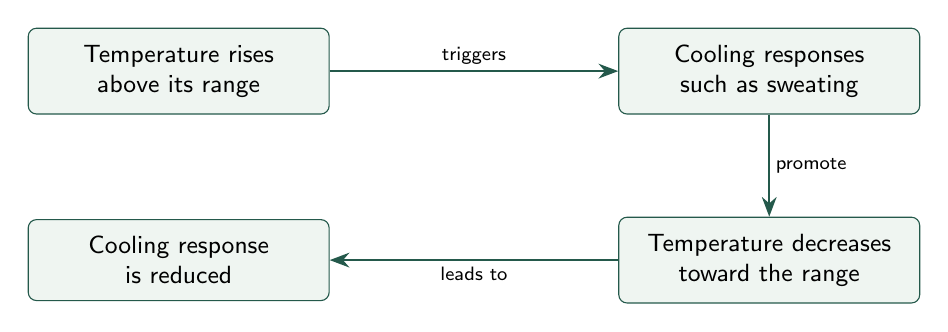
\begin{tikzpicture}
\node[concept] (a) at (0,0) {Temperature rises\\above its range};
\node[concept] (b) at (7.5,0) {Cooling responses\\such as sweating};
\node[concept] (c) at (7.5,-2.4) {Temperature decreases\\toward the range};
\node[concept] (d) at (0,-2.4) {Cooling response\\is reduced};
\draw[flow] (a)--node[rel,above]{triggers}(b);
\draw[flow] (b)--node[rel,right]{promote}(c);
\draw[flow] (c)--node[rel,below]{leads to}(d);
\end{tikzpicture}\par
\end{center}
\textbf{Negative feedback} opposes the initiating change. As temperature returns toward its regulated range, the corrective response is reduced. \textbf{Positive feedback} amplifies a change, as contractions promote signals that strengthen contractions during childbirth until delivery ends the loop. ``Positive'' and ``negative'' describe direction, not whether a response is helpful or harmful.

\textbf{Experimental control} provides a comparison condition. \textbf{Constants} are factors kept the same. In a temperature experiment, control food and water so their effects are not confused with temperature's effects.
\memorycheck{If temperature falls and shivering raises it, which feedback type is operating? Explain using the initial change and the response.}

\pagechapter{1B\quad The characteristics of life}{lifecheck}
\idea{A living organism is an organized cellular system. No single sign, such as movement or growth, is enough to identify life.}
\par
\begin{tabularx}{\linewidth}{@{}p{0.26\linewidth}Y@{}}\toprule
Characteristic & Meaning and a useful example\\\midrule
Made of cells & Cells are the basic units of life. A bacterium is unicellular; a tree is multicellular.\\
Reproduction & Organisms produce offspring through a life cycle or lineage. A sterile individual can still be alive.\\
Genetic information & DNA stores inherited information; RNA helps cells use that information. Offspring inherit information from parents.\\
Growth and development & Growth increases size or cell number. Development changes form or function, such as a seedling forming mature leaves.\\
Matter and energy use & Metabolic reactions supply materials and usable energy for cellular work. A plant takes in carbon dioxide and captures light energy.\\
Response to stimuli & A stimulus is a change an organism detects. A plant growing toward light is a response; walking is not required.\\
Homeostasis & Organisms regulate internal conditions within functional ranges even while the surroundings change.\\
Evolution & Inherited characteristics of populations change across generations. An individual does not evolve during its lifetime.\\\bottomrule
\end{tabularx}\par
\subsection*{Apply the whole checklist}
\textbf{Fire} spreads, uses fuel, and releases heat, but has no cells or biological genetic system. \textbf{A dormant seed} may show little visible activity, but contains living cells and can resume growth under suitable conditions. \textbf{A sterile mule} is alive despite its inability to reproduce.
\subsection*{Metabolism connects the characteristics}
Building molecules supports growth and repair. Breaking down fuel molecules can transfer energy to ATP. ATP supports movement, synthesis, and transport across membranes. These processes help cells maintain homeostasis.

\textbf{Do not confuse terms.} Metabolism is the collection of chemical reactions; homeostasis is regulation of conditions. Respiration is one metabolic process that helps supply energy for regulation. The class's example of a room warming when people enter connects cellular respiration to heat released into the surroundings.
\memorycheck{Explain why a feather is biologically derived material but is not itself a living organism.}
\classsource{Lecture 1 What Is Life Skeleton Notes; Metabolism, Trophic Levels and Energy Transfer, slides 2 and 5--7.}

\pagechapter{1B\quad Cells and viruses}{cells}
\idea{Viruses share genetic information and evolution with living systems, but lack the independent cellular organization used in the class's life checklist.}
\begin{center}
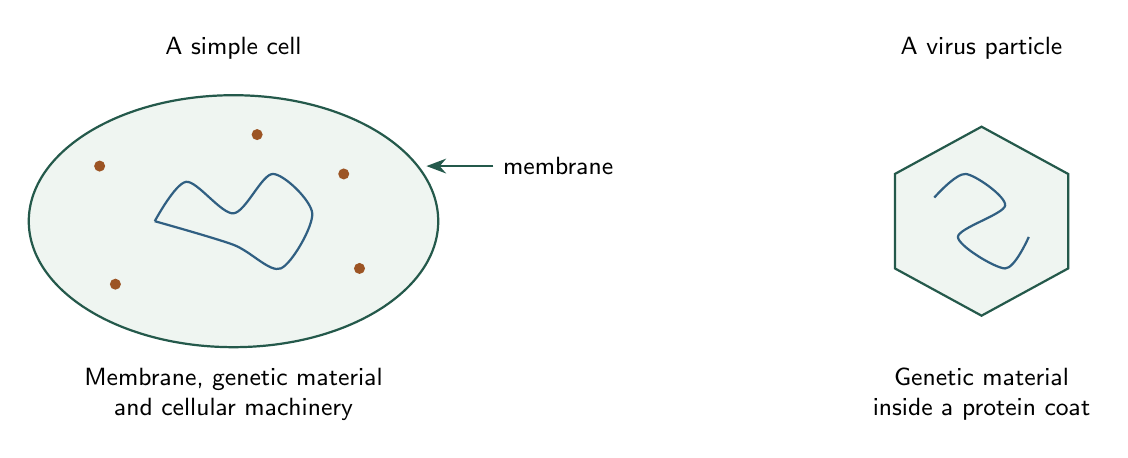
\begin{tikzpicture}[font=\small\sffamily]
\draw[thick,forest,fill=pale] (0,0) ellipse (2.6 and 1.6);
\draw[blue,thick] plot[smooth] coordinates {(-1,0)(-0.6,0.5)(0,0.1)(0.5,0.6)(1,0.1)(0.6,-0.6)(0,-0.3)(-1,0)};
\foreach \x/\y in {-1.7/0.7,-1.5/-0.8,1.4/0.6,1.6/-0.6,0.3/1.1} {\fill[orange] (\x,\y) circle (0.07);}
\node at (0,2.2) {A simple cell};
\node[align=center] at (0,-2.2) {Membrane, genetic material\\and cellular machinery};
\draw[flow] (3.3,0.7)--(2.45,0.7);
\node[anchor=west] at (3.3,0.7) {membrane};
\begin{scope}[xshift=9.5cm]
\draw[thick,forest,fill=pale] (0,1.2)--(1.1,0.6)--(1.1,-0.6)--(0,-1.2)--(-1.1,-0.6)--(-1.1,0.6)--cycle;
\draw[blue,thick] plot[smooth] coordinates {(-0.6,0.3)(-0.2,0.6)(0.3,0.2)(-0.3,-0.2)(0.3,-0.6)(0.6,-0.2)};
\node at (0,2.2) {A virus particle};
\node[align=center] at (0,-2.2) {Genetic material\\inside a protein coat};
\end{scope}
\end{tikzpicture}\par
\end{center}
\textit{Schematic, not to scale.} The blue line represents genetic material; the cell's orange dots represent ribosomes. Shapes vary, and some viruses also have an envelope.
\par
\begin{tabularx}{\linewidth}{@{}p{0.25\linewidth}Y Y@{}}\toprule
Feature & Cellular organism & Virus\\\midrule
Organization & One or more cells & Not made of cells\\
Genome & DNA & DNA or RNA\\
Metabolism & Has cellular metabolism & Lacks an independent metabolic system\\
Making copies & Uses cellular machinery & Requires a host cell's machinery\\
Evolution & Populations evolve & Viral populations evolve too\\\bottomrule
\end{tabularx}\par
\subsection*{How to answer the classification question}
State the criteria, then apply them. Under the usual school biology criteria, viruses are classified as nonliving because they are not cellular and cannot independently carry out metabolism or make new particles. Their genetic information and capacity to evolve explain why the comparison is interesting.

The viral coat helps protect the genome and, through viral surface structures, enables attachment to suitable host cells. A host cell supplies machinery and resources used to assemble new virus particles. A virus does not simply grow and divide like a cell.
\memorycheck{Why does requiring a host's cellular machinery matter more than simply requiring food from the environment?}
\classsource{Lecture 1 What Is Life Skeleton Notes, virus questions. Verification: \href{https://openstax.org/books/biology-2e/pages/21-introduction}{OpenStax Biology 2e, Viruses}.}

\pagechapter{1B\quad Drawing feedback loops}{feedback}
\idea{Track one measurable condition. Negative feedback opposes its change; positive feedback reinforces it. The sign describes a relationship, not whether a response is helpful.}
\subsection*{Temperature regulation in both directions}
\begin{center}
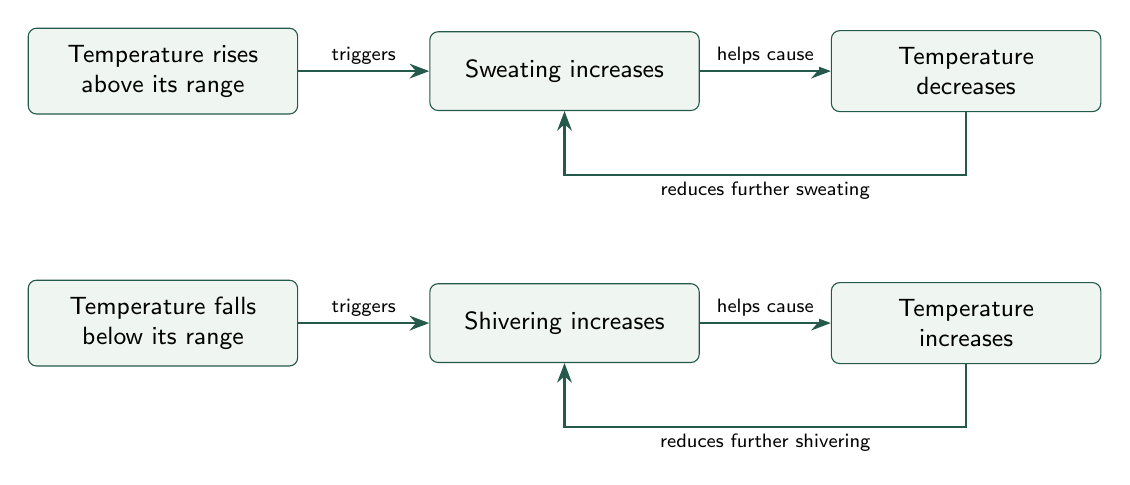
\begin{tikzpicture}[concept/.append style={text width=3cm}]
\node[concept] (hot) at (0,0) {Temperature rises above its range};
\node[concept] (sweat) at (5.1,0) {Sweating increases};
\node[concept] (down) at (10.2,0) {Temperature decreases};
\draw[flow] (hot)--node[rel,above]{triggers}(sweat);
\draw[flow] (sweat)--node[rel,above]{helps cause}(down);
\draw[flow] (down.south)--++(0,-0.8)-|node[rel,pos=0.25,below]{reduces further sweating}(sweat.south);
\node[concept] (cold) at (0,-3.2) {Temperature falls below its range};
\node[concept] (shiver) at (5.1,-3.2) {Shivering increases};
\node[concept] (up) at (10.2,-3.2) {Temperature increases};
\draw[flow] (cold)--node[rel,above]{triggers}(shiver);
\draw[flow] (shiver)--node[rel,above]{helps cause}(up);
\draw[flow] (up.south)--++(0,-0.8)-|node[rel,pos=0.25,below]{reduces further shivering}(shiver.south);
\end{tikzpicture}\par
\end{center}
Sweat evaporation transfers heat away from the body. Shivering uses repeated muscle contractions; greater energy use and metabolism release more heat. Recovery toward the regulated range reduces corrective action.
\subsection*{A self-reinforcing loop}
\begin{center}
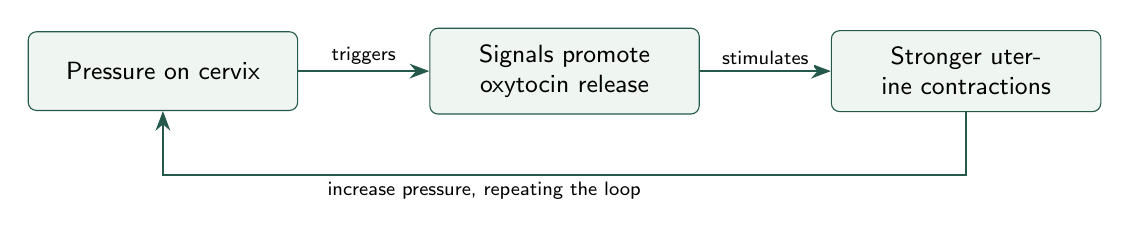
\begin{tikzpicture}[concept/.append style={text width=3cm}]
\node[concept] (p) at (0,0) {Pressure on cervix};
\node[concept] (s) at (5.1,0) {Signals promote oxytocin release};
\node[concept] (c) at (10.2,0) {Stronger uterine contractions};
\draw[flow] (p)--node[rel,above]{triggers}(s);
\draw[flow] (s)--node[rel,above]{stimulates}(c);
\draw[flow] (c.south)--++(0,-0.8)-|node[rel,pos=0.3,below]{increase pressure, repeating the loop}(p.south);
\end{tikzpicture}\par
\end{center}
Delivery removes the initiating pressure. A chain that never returns to affect the original condition is not a complete feedback explanation.
\memorycheck{Choose an everyday condition, draw a response, and show how it changes the same condition.}
\classsource{Feedback Mechanisms and Homeostasis, slides 2--5; Feedback Mechanisms and Homestasis Practice.}


\pagechapter{1C\quad Energy and matter in ecosystems}{onec}
\idea{Energy passes through ecosystems and dissipates as heat. Matter is transferred and recycled through organisms and their surroundings.}
\subsection*{The parts of an ecosystem}
An \textbf{ecosystem} includes organisms, the physical environment, and their interactions. \textbf{Biotic} components involve life, including organisms and biologically derived material such as dead leaves in the class convention. \textbf{Abiotic} factors include temperature, light, humidity, water, and minerals.

A \textbf{habitat} is where an organism lives. Its \textbf{niche} includes how it uses resources, the conditions it tolerates, and its interactions. A pond is a frog's habitat; consuming insects and serving as prey are parts of its niche.
\par
\begin{tabularx}{\linewidth}{@{}p{0.28\linewidth}Y@{}}\toprule
Role & How matter and energy are obtained\\\midrule
Autotroph or producer & Builds organic molecules from inorganic carbon using light or chemical energy. Plants are familiar photosynthetic producers.\\
Heterotroph or consumer & Obtains organic matter from other organisms or their products. Animals, fungi, and many microbes are heterotrophs.\\
Decomposer & Breaks down dead organic material and wastes, returning nutrients to forms that can reenter ecosystem cycles. Many fungi and bacteria do this.\\\bottomrule
\end{tabularx}
\par
Most food webs rely on sunlight. Some producers use \textbf{chemosynthesis}, obtaining energy from chemical reactions involving inorganic substances rather than light. Lack of oxygen is not the defining feature.
\subsection*{Two processes to connect}
Simplified overall equations for oxygen-producing photosynthesis and aerobic cellular respiration are:
\begin{align*}
\text{Photosynthesis:}\quad 6\mathrm{CO_2}+6\mathrm{H_2O}+\text{light}
&\longrightarrow \mathrm{C_6H_{12}O_6}+6\mathrm{O_2}\\
\text{Respiration:}\quad \mathrm{C_6H_{12}O_6}+6\mathrm{O_2}
&\longrightarrow 6\mathrm{CO_2}+6\mathrm{H_2O}+\text{energy transfer}
\end{align*}
Photosynthesis stores transferred light energy in organic molecules. Respiration transfers chemical energy to ATP and releases heat. \textbf{Plants perform cellular respiration too.} ATP supports cellular work, including processes needed for homeostasis.

Atoms are rearranged in these reactions; energy is not turned into matter, and matter does not disappear into energy. Decomposers also metabolize and respire; they do not recycle heat into sunlight.
\memorycheck{Trace one carbon atom and the energy associated with food through a plant, a rabbit, and a decomposer. How do their paths differ?}

\pagechapter{1C\quad Reading a food web}{web}
\idea{A food-web arrow points from a food source to the organism receiving its matter and chemical energy.}
\begin{center}
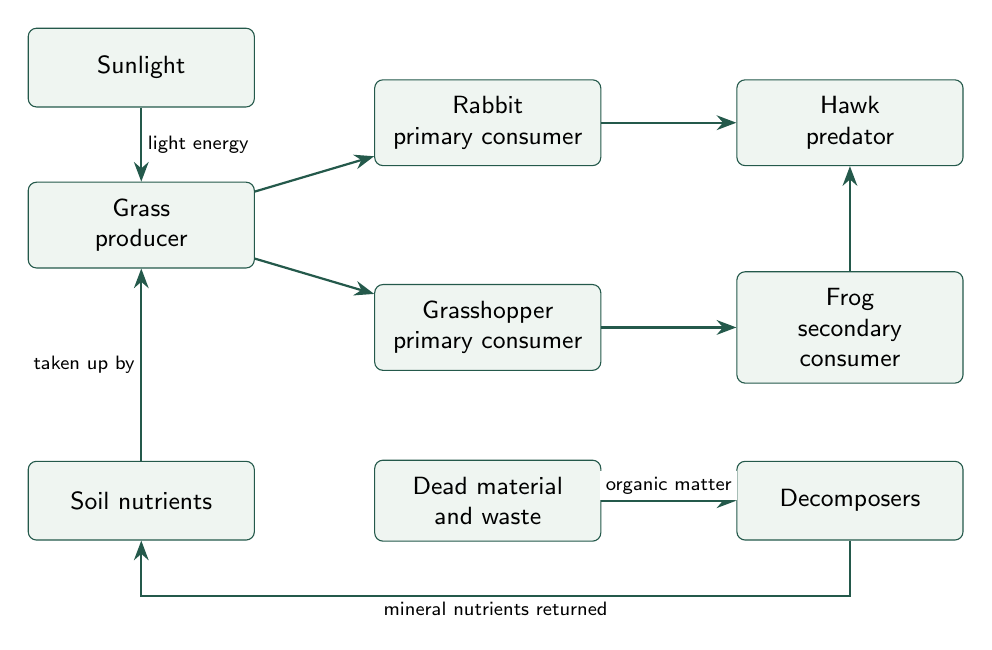
\begin{tikzpicture}[concept/.append style={text width=2.45cm}]
\node[concept] (sun) at (0,0) {Sunlight};
\node[concept] (grass) at (0,-2) {Grass\\producer};
\node[concept] (rabbit) at (4.4,-0.7) {Rabbit\\primary consumer};
\node[concept] (insect) at (4.4,-3.3) {Grasshopper\\primary consumer};
\node[concept] (hawk) at (9,-0.7) {Hawk\\predator};
\node[concept] (frog) at (9,-3.3) {Frog\\secondary consumer};
\node[concept] (dead) at (4.4,-5.5) {Dead material\\and waste};
\node[concept] (dec) at (9,-5.5) {Decomposers};
\node[concept] (soil) at (0,-5.5) {Soil nutrients};
\draw[flow] (sun)--node[rel,right]{light energy}(grass);
\draw[flow] (grass)--(rabbit);
\draw[flow] (grass)--(insect);
\draw[flow] (rabbit)--(hawk);
\draw[flow] (insect)--(frog);
\draw[flow] (frog)--(hawk);
\draw[flow] (dead)--node[rel,above]{organic matter}(dec);
\draw[flow] (dec.south) -- ++(0,-0.7) -| node[rel,pos=0.25,below]{mineral nutrients returned}(soil.south);
\draw[flow] (soil)--node[rel,left]{taken up by}(grass);
\end{tikzpicture}\par
\end{center}
All organisms contribute dead material or waste to the decomposer pathway; those arrows are omitted for clarity. Feeding arrows are unlabeled. Other arrows state the process represented. All living groups release metabolic heat, which leaves the food web as usable energy decreases.

\textbf{Trophic level} means feeding position. The hawk is a secondary consumer when eating a rabbit and a tertiary consumer when eating a frog that ate a grasshopper. An organism can occupy more than one trophic level.
\subsection*{Predict a change by following the links}
\begin{itemize}
\item \textbf{Remove producers:} the food supply to herbivores declines, and effects pass to predators. Existing stored food or imported organic matter can delay the response.
\item \textbf{Remove decomposers:} dead material accumulates and nutrient recycling slows; producer growth can eventually be limited.
\item \textbf{Remove top predators:} some prey may increase and consume more of their food. The size and timing of the response depend on alternative prey, competition, and other limits.
\end{itemize}
\memorycheck{Why does removing frogs not guarantee an immediate hawk decline in this web? State an alternative food source and a remaining uncertainty.}

\pagechapter{1C\quad Diagramming energy and gases}{gases}
\idea{Separate energy transfers from gas exchange. Gases enter or leave the surroundings rather than passing along feeding arrows.}
\subsection*{Energy pathway}
\begin{center}
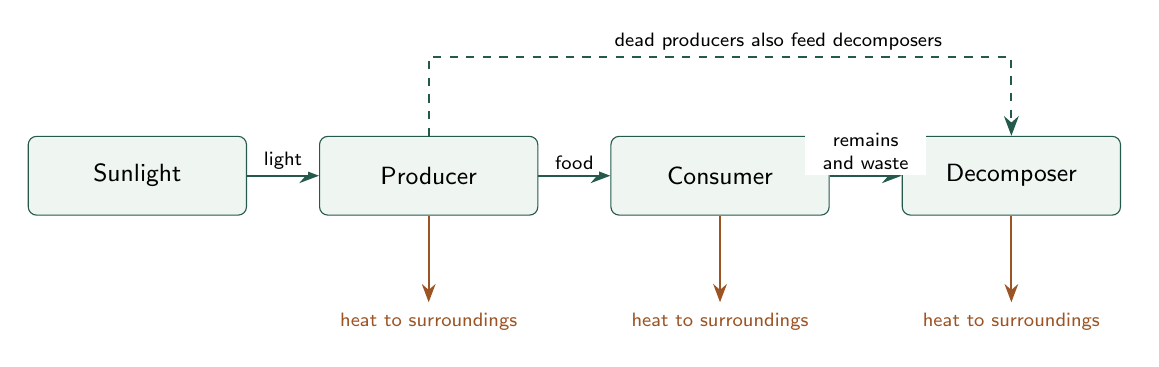
\begin{tikzpicture}[concept/.append style={text width=2.35cm}]
\node[concept] (sun) at (0,0) {Sunlight};
\node[concept] (plant) at (3.7,0) {Producer};
\node[concept] (animal) at (7.4,0) {Consumer};
\node[concept] (decomp) at (11.1,0) {Decomposer};
\draw[flow] (sun)--node[rel,above]{light}(plant);
\draw[flow] (plant)--node[rel,above]{food}(animal);
\draw[flow] (animal)--node[rel,above,text width=1.4cm]{remains\\and waste}(decomp);
\foreach \a in {plant,animal,decomp} {
\draw[-{Stealth},thick,orange] (\a.south)--++(0,-1.1) node[below,font=\scriptsize\sffamily,text width=2.8cm,align=center]{heat to surroundings};
}
\draw[flow,dashed] (plant.north)--++(0,1)-|node[rel,pos=0.3,above]{dead producers also feed decomposers}(decomp.north);
\end{tikzpicture}\par
\end{center}
Photosynthesis converts light to chemical energy. Feeding transfers organic molecules and their chemical energy. Cellular respiration transfers energy to ATP, while metabolic processes release heat. Decomposers receive remains from any trophic level.
\subsection*{Gas exchange with the surroundings}
\begin{center}
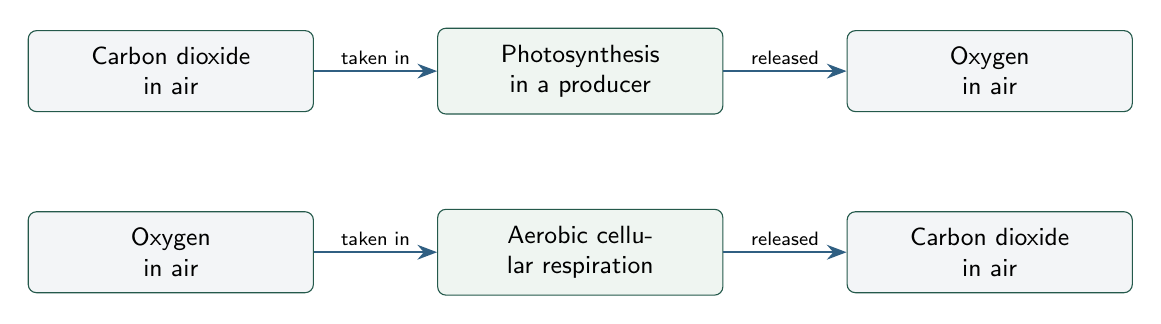
\begin{tikzpicture}[concept/.append style={text width=3.2cm}]
\node[concept,fill=blue!6] (co) at (0,0) {Carbon dioxide\\in air};
\node[concept] (photo) at (5.2,0) {Photosynthesis\\in a producer};
\node[concept,fill=blue!6] (ox) at (10.4,0) {Oxygen\\in air};
\draw[flow,blue] (co)--node[rel,above]{taken in}(photo);
\draw[flow,blue] (photo)--node[rel,above]{released}(ox);
\node[concept,fill=blue!6] (ox2) at (0,-2.3) {Oxygen\\in air};
\node[concept] (resp) at (5.2,-2.3) {Aerobic cellular respiration};
\node[concept,fill=blue!6] (co2) at (10.4,-2.3) {Carbon dioxide\\in air};
\draw[flow,blue] (ox2)--node[rel,above]{taken in}(resp);
\draw[flow,blue] (resp)--node[rel,above]{released}(co2);
\end{tikzpicture}\par
\end{center}
The respiration row applies to plants, animals, and aerobic decomposers. Plants need both sets of gas arrows. Aquatic organisms may exchange dissolved gases with water rather than directly with air.
\textbf{Decomposition} acts on dead material; the decomposer uses its own metabolism. Some microbes use pathways without oxygen, so the aerobic row does not represent every microbe.
\memorycheck{Draw a plant, a rabbit, and aerobic decomposers. Add food, heat, and gas arrows for every relevant process.}
\classsource{Metabolism, Trophic Levels and Energy Transfer, slides 2--7 and 19--27; Energy, Ecosystems, and Ecology Part 1; Energy and Matter Language Guide.}

\pagechapter{1C\quad Consumer roles and energy language}{roles}
\idea{Feeding role describes how an organism obtains organic matter. Trophic level describes its position in a particular feeding pathway.}
\par
\begin{tabularx}{\linewidth}{@{}p{0.25\linewidth}Y Y@{}}\toprule
Role & Definition & Example\\\midrule
Herbivore & Eats plants or algae & Rabbit eating grass\\
Carnivore & Eats animals & Hawk eating a rabbit\\
Omnivore & Eats plant and animal material & Bear eating berries and fish\\
Scavenger & Consumes remains of dead animals & Vulture feeding on a carcass\\
Detritivore & Ingests small pieces of dead organic matter & Earthworm eating organic material in soil\\
Decomposer & Breaks down organic matter externally and absorbs products & Fungus growing on dead wood\\\bottomrule
\end{tabularx}\par
These categories can overlap. Detritivores physically process material; microbial decomposers chemically break it down and return nutrients to reusable forms. Decomposers are heterotrophs, not producers.
\subsection*{Trace the molecules and the energy separately}
\textbf{Digestion} breaks food into smaller molecules that can be absorbed. \textbf{Cellular respiration} processes fuel molecules in cells, transferring chemical energy to ATP. \textbf{ATP} provides an immediate energy supply for muscle contraction, molecule synthesis, and transport across membranes.

Plants obtain most of the carbon in their organic molecules from carbon dioxide. Fertilizer supplies mineral nutrients; it does not supply the sunlight captured in photosynthesis. Water and minerals contribute matter, while light supplies energy.

\textbf{Say:} organisms obtain, store, convert, transfer, or release energy. Avoid saying organisms create energy or that glucose simply becomes ATP. During respiration, energy is transferred to ATP while atoms from fuel molecules are rearranged into products.
\subsection*{Worked comparison}
A wood-burning stove and a person both use energy stored in organic matter and release heat. In the person, cellular pathways also transfer energy to ATP for regulated cellular work. The stove does not have cells, homeostasis, or biological reproduction.

Shivering connects the same ideas: muscle contraction uses ATP, metabolism supplies usable energy, and heat release helps raise body temperature. Increased metabolic rate means more reactions per unit time, not the creation of new energy.
\memorycheck{Why is a mushroom a heterotroph even though it never chases prey?}
\classsource{Metabolism, Trophic Levels and Energy Transfer, slides 12--20; Trophic Levels Skeleton Notes; Energy and Matter Language Guide and questions; Energy and Matter Practice Questions.}

\pagechapter{1C\quad The energy-flow lab}{lab}
\idea{Compare water-temperature changes across control, still-hand, and moving-hand conditions, then explain the energy pathway.}
\begin{center}
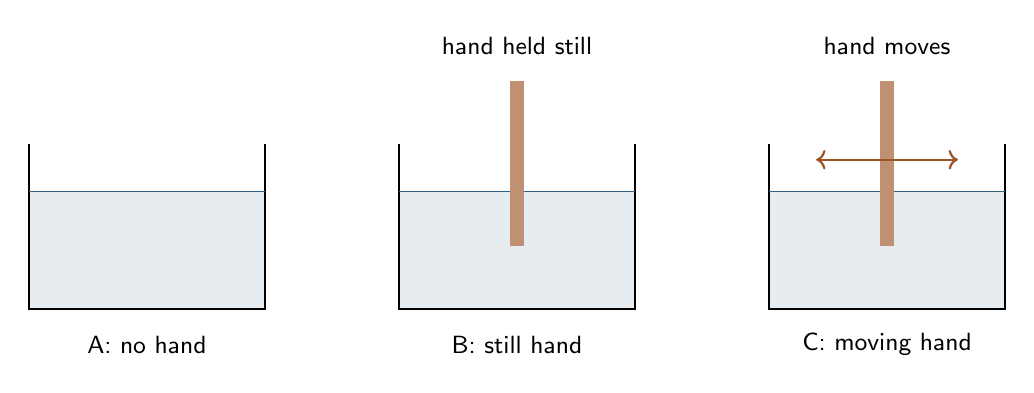
\begin{tikzpicture}[font=\small\sffamily]
\foreach \x/\lab in {0/A: no hand,4.7/B: still hand,9.4/C: moving hand} {
\fill[blue!12] (\x,0) rectangle ++(3,1.5);
\draw[thick] (\x,2.1)--(\x,0)--++(3,0)--++(0,2.1);
\draw[blue] (\x,1.5)--++(3,0);
\node at (\x+1.5,-0.45) {\lab};
}
\draw[line width=5pt,orange!65] (6.2,2.9)--(6.2,0.8);
\draw[line width=5pt,orange!65] (10.9,2.9)--(10.9,0.8);
\draw[<->,thick,orange] (10,1.9)--(11.8,1.9);
\node at (6.2,3.35) {hand held still};
\node at (10.9,3.35) {hand moves};
\end{tikzpicture}\par
\end{center}
\textit{Setup schematic.} Colored bars represent hands, not thermometers. The handout uses a 500-ml bottle of water for each container and records temperature initially and once each minute for five minutes.
\begin{center}
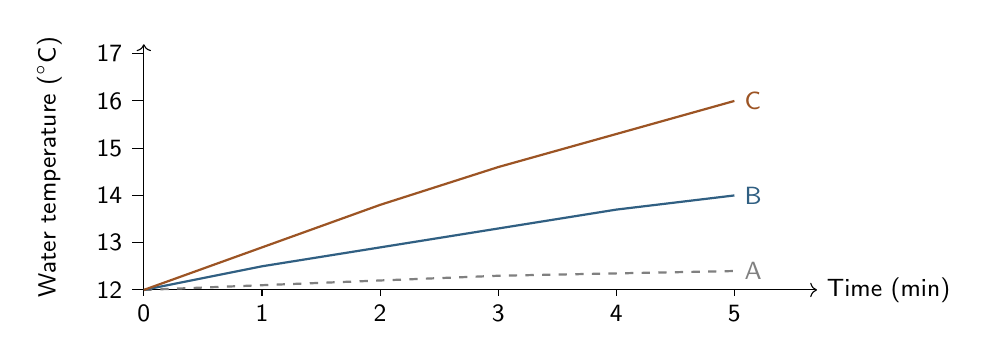
\begin{tikzpicture}[x=1.5cm,y=0.60cm,font=\small\sffamily]
\draw[->] (0,0)--(5.7,0) node[right]{Time (min)};
\draw[->] (0,0)--(0,5.2);
\node[rotate=90] at (-0.8,2.6) {Water temperature ($^\circ$C)};
\foreach \x in {0,1,2,3,4,5} {\draw (\x,0)--(\x,-0.12) node[below]{\x};}
\foreach \y/\lab in {0/12,1/13,2/14,3/15,4/16,5/17} {\draw (0,\y)--(-0.1,\y) node[left]{\lab};}
\draw[gray,thick,dashed] plot coordinates {(0,0)(1,0.1)(2,0.2)(3,0.3)(4,0.35)(5,0.4)} node[right]{A};
\draw[blue,thick] plot coordinates {(0,0)(1,0.5)(2,0.9)(3,1.3)(4,1.7)(5,2)} node[right]{B};
\draw[orange,thick] plot coordinates {(0,0)(1,0.9)(2,1.8)(3,2.6)(4,3.3)(5,4)} node[right]{C};
\end{tikzpicture}\par
\end{center}
\textbf{Invented practice data, not Shawn's results.} Changes are A: $0.4^\circ$C, B: $2.0^\circ$C, C: $4.0^\circ$C. A shows warming possible without a hand. Initial temperatures, hand size, movement, and timing are potential sources of variability.
\textbf{Heat calculation.} The handout's approximation for water is:
\[
Q\;(\mathrm{Cal})=V\;(\mathrm{L})\times\Delta T\;({}^\circ\mathrm C).
\]
For 0.50 L warmed by $4.0^\circ$C, $Q=2.0$ Cal, or 2 kcal. This is heat gained by the water, not all energy used by the body. Movement also affects mixing and heat transfer, so water warming does not isolate metabolic heat production.
\classsource{Energy Flow Lab 2021, procedure and quantitative questions; Energy and Matter Language Guide.}


\pagechapter{1C\quad Ecological pyramids}{pyramids}
\idea{Less energy is available to support production at successively higher trophic levels. This constrains food-chain length and predator populations.}
\begin{center}
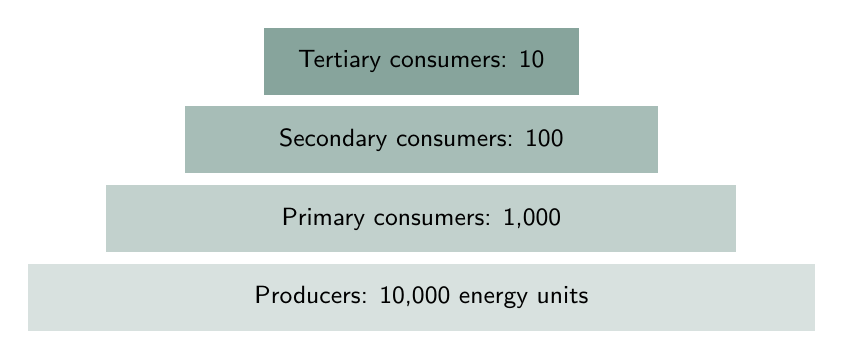
\begin{tikzpicture}[font=\small\sffamily]
\fill[forest!18] (-5,0) rectangle (5,0.85);
\fill[forest!28] (-4,1) rectangle (4,1.85);
\fill[forest!40] (-3,2) rectangle (3,2.85);
\fill[forest!55] (-2,3) rectangle (2,3.85);
\node at (0,0.42) {Producers: 10,000 energy units};
\node at (0,1.42) {Primary consumers: 1,000};
\node at (0,2.42) {Secondary consumers: 100};
\node at (0,3.42) {Tertiary consumers: 10};
\end{tikzpicture}\par
\end{center}
\textit{Illustration only:} values assume 10\% transfer at each step, use the same area and time interval, and are not measured data. Rectangle widths are schematic, not proportional to the numbers.

The \textbf{10\% rule} is a useful classroom approximation, not a fixed efficiency for every ecosystem. Energy not passed to the next consumer level can go into respiration and heat, uneaten material, or waste. Energy in detritus can still support decomposers before eventually dissipating as heat.
\[
E_{\text{next}}=E_{\text{current}}\times\text{transfer fraction}
\]
For an assumed 10\% transfer, two steps above 10,000 units gives
$10{,}000\times0.10\times0.10=100$ units.
\subsection*{Do not confuse three types of pyramid}
\begin{itemize}
\item \textbf{Energy:} energy transfer or production per area per time; an upright pattern is expected across a food chain.
\item \textbf{Biomass:} mass of organisms present; a snapshot can be inverted when rapidly reproducing producers are consumed quickly.
\item \textbf{Numbers:} count of organisms; one large tree can support many insects, so counts need not decrease at every level.
\end{itemize}
\subsection*{Why top predators are vulnerable}
\textbf{First,} limited energy supports relatively few predators, making small populations vulnerable to additional losses. \textbf{Second,} predators depend on a broad supporting prey base and often need large areas, making habitat loss and disruption below them consequential. \textbf{An additional risk} is biomagnification: some persistent pollutants reach higher concentrations up food chains.
\source{OpenStax, \href{https://openstax.org/books/biology-2e/pages/46-2-energy-flow-through-ecosystems}{Energy Flow through Ecosystems}, for pyramid exceptions and transfer efficiency.}
\memorycheck{Explain why ``the missing 90\% was destroyed'' is incorrect.}

\pagechapter{2A\quad Biodiversity and ecosystem services}{twoa}
\idea{Variety within and among living systems can help ecosystem functions persist through change and provides benefits people rely on.}
\subsection*{Three scales of biodiversity}
\begin{itemize}
\item \textbf{Genetic diversity:} inherited variation within a species, such as different alleles affecting disease resistance.
\item \textbf{Species diversity:} variety of species in a community; both species richness and their relative abundances matter.
\item \textbf{Ecosystem diversity:} variety of ecosystems, such as wetlands, forests, and grasslands across a region.
\end{itemize}
\textbf{Resilience} is the capacity to recover or retain functions after disturbance. If several pollinators respond differently to drought, some may keep pollinating when others decline. Diversity often helps, but does not guarantee recovery from every disturbance. Species roles and the severity of change also matter.
\begin{center}
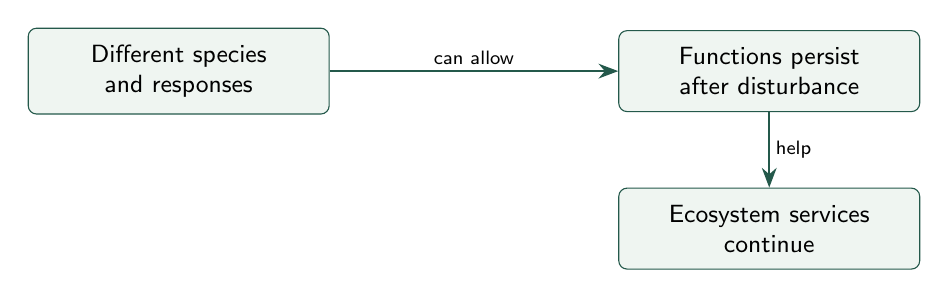
\begin{tikzpicture}
\node[concept] (a) at (0,0) {Different species\\and responses};
\node[concept] (b) at (7.5,0) {Functions persist\\after disturbance};
\node[concept] (c) at (7.5,-2) {Ecosystem services\\continue};
\draw[flow] (a)--node[rel,above]{can allow}(b);
\draw[flow] (b)--node[rel,right]{help}(c);
\end{tikzpicture}\par
\end{center}
\subsection*{Ecosystem services are benefits to people}
Food, materials, water filtration, flood buffering, pollination, nutrient cycling, recreation, and cultural value connect ecosystem processes to human needs. \textbf{Pollination} transfers pollen to a receptive reproductive structure and enables fertilization in many plants.

The supplied Biodiversity Worksheet asks for all four categories, so learn each definition and be able to provide examples:
\par
\begin{tabularx}{\linewidth}{@{}p{0.25\linewidth}Y@{}}\toprule
Category & Examples\\\midrule
Provisioning & Food, timber, and other biological materials\\
Regulating & Flood moderation, water purification, crop pollination\\
Supporting & Nutrient cycling and soil formation\\
Cultural & Recreation, scenic enjoyment, spiritual significance\\\bottomrule
\end{tabularx}
\par
\textbf{Keystone species.} A species whose effect on community structure is unusually large relative to its abundance. Some predators have this role, but not every predator is a keystone species.
\memorycheck{Explain how losing pollinators can affect plants, other animals, and humans.}

\pagechapter{2A\quad Seeing biodiversity at three scales}{diversity}
\idea{Genetic, species, and ecosystem diversity describe different levels. State which level your evidence measures.}
\begin{center}
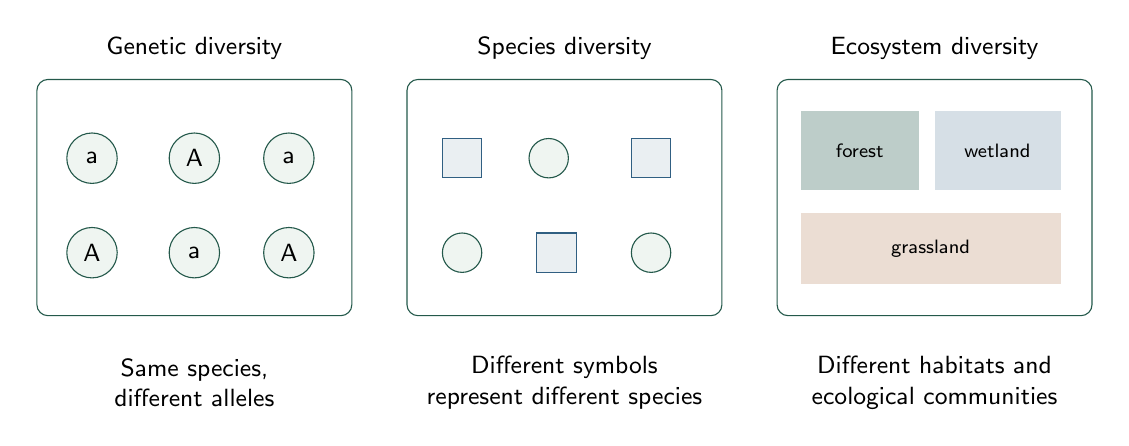
\begin{tikzpicture}[font=\small\sffamily]
\foreach \x/\title in {0/Genetic diversity,4.7/Species diversity,9.4/Ecosystem diversity} {
\draw[forest,rounded corners] (\x,0) rectangle ++(4,3);
\node at (\x+2,3.4) {\title};
}
\foreach \x/\y/\lab in {0.7/0.8/A,2/0.8/a,3.2/0.8/A,0.7/2/a,2/2/A,3.2/2/a} {
\draw[forest,fill=pale] (\x,\y) circle (0.32);
\node at (\x,\y) {\lab};
}
\foreach \x/\y in {5.4/0.8,6.5/2,7.8/0.8} {\draw[forest,fill=pale] (\x,\y) circle (0.25);}
\foreach \x/\y in {5.4/2,6.6/0.8,7.8/2} {\draw[blue,fill=blue!10] (\x-0.25,\y-0.25) rectangle ++(0.5,0.5);}
\fill[forest!30] (9.7,1.6) rectangle ++(1.5,1);
\fill[blue!20] (11.4,1.6) rectangle ++(1.6,1);
\fill[orange!20] (9.7,0.4) rectangle ++(3.3,0.9);
\node[font=\scriptsize\sffamily] at (10.45,2.1) {forest};
\node[font=\scriptsize\sffamily] at (12.2,2.1) {wetland};
\node[font=\scriptsize\sffamily] at (11.35,0.85) {grassland};
\node[align=center,text width=4cm] at (2,-0.85) {Same species,\\different alleles};
\node[align=center,text width=4cm] at (6.7,-0.85) {Different symbols\\represent different species};
\node[align=center,text width=4cm] at (11.4,-0.85) {Different habitats and\\ecological communities};
\end{tikzpicture}\par
\end{center}
Letters represent schematic alleles, not complete genotypes. Genetic variation can increase the chance that some individuals tolerate a change. It cannot guarantee that a helpful trait exists or that every individual survives.
\subsection*{Why species roles matter}
A \textbf{keystone species} has an unusually large effect relative to its abundance. Some predators regulate prey and thereby influence vegetation and other organisms. The effect depends on the food web; not every predator is a keystone species.

The worksheet asks why corals matter. Reef-building corals create physical habitat used for shelter and feeding. Losing reef structure can affect many species. This habitat-building role is often described more precisely as a \textbf{foundation species} role.
\begin{center}
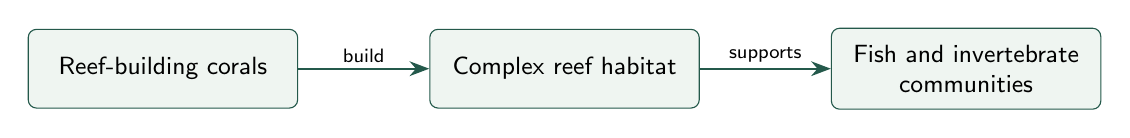
\begin{tikzpicture}[concept/.append style={text width=3cm}]
\node[concept] (c) at (0,0) {Reef-building corals};
\node[concept] (h) at (5.1,0) {Complex reef habitat};
\node[concept] (f) at (10.2,0) {Fish and invertebrate communities};
\draw[flow] (c)--node[rel,above]{build}(h);
\draw[flow] (h)--node[rel,above]{supports}(f);
\end{tikzpicture}\par
\end{center}
\textbf{Services connect mechanisms to people.} Fish are provisioning resources; water purification is regulating; nutrient cycling is supporting; recreation and cultural meaning are cultural benefits. Explain both the category and the process.
\memorycheck{Does a forest with many trees, all of one species, necessarily have high tree species diversity?}
\classsource{Biodiversity Worksheet; Biodiversity and Its Threats Debrief, slides 2--6. Coral clarification: \href{https://coralreef.noaa.gov/digital-corals/visual-media/infographics/corals-are-important}{NOAA, Corals are Important}.}


\pagechapter{2B\quad Threats to biodiversity}{twob}
\idea{Human activities change habitats, resources, and interactions. Conservation works best when it addresses the specific cause of decline.}
The practice key expands \textbf{CHIPPO} as follows:
\par
\begin{tabularx}{\linewidth}{@{}p{0.25\linewidth}Y@{}}\toprule
Threat & Mechanism and a possible response\\\midrule
Climate change & Shifts temperature, rainfall, and habitat suitability. Reduce emissions and protect routes for species movement.\\
Habitat loss & Farming, buildings, roads, logging, and mining can remove or degrade habitat. Protect and restore suitable habitat.\\
Invasive species & Introduced species can spread and harm native species through competition, predation, or disease. Prevent introductions and manage established invasions.\\
Pollution & Chemicals, nutrient excess, plastics, and other pollutants can impair organisms or habitats. Reduce releases at their source.\\
Population & Human population size interacts with consumption and technology to influence resource demand. Improve access to resources and reduce waste and damaging demand.\\
Overexploitation & Harvest exceeds a population's capacity to replace losses. Use sustainable harvest limits and protect breeding populations.\\\bottomrule
\end{tabularx}
\par
\textbf{Overconsumption} means resource use beyond what is needed or can be sustained. Population alone does not determine impact: per-person use and production methods also matter. \textbf{Endangered} species face a high risk of extinction; an \textbf{extinct} species has no living individuals remaining.
\subsection*{Habitat loss versus fragmentation}
\textbf{Loss} reduces the amount of habitat. \textbf{Fragmentation} divides habitat into separated patches. The same development can do both. Isolation can limit migration and mating, reduce gene flow, increase edge exposure, and make local losses harder to reverse.
\begin{center}
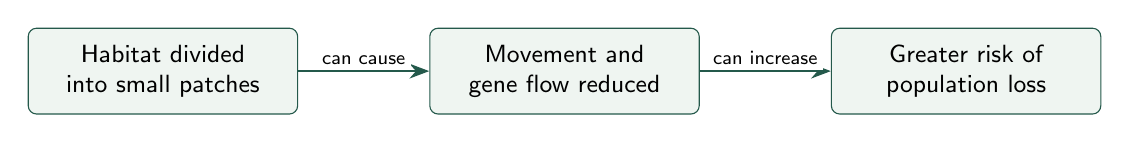
\begin{tikzpicture}[concept/.append style={text width=3cm}]
\node[concept] (a) at (0,0) {Habitat divided\\into small patches};
\node[concept] (b) at (5.1,0) {Movement and\\gene flow reduced};
\node[concept] (c) at (10.2,0) {Greater risk of\\population loss};
\draw[flow] (a)--node[rel,above]{can cause}(b);
\draw[flow] (b)--node[rel,above]{can increase}(c);
\end{tikzpicture}\par
\end{center}
\textbf{Wildlife corridors} connect patches and can improve movement. Their benefits depend on design and species; connecting patches does not replace all lost habitat. An introduced species is not automatically invasive: harmful effects matter.\footnote{See \href{https://www.cbd.int/invasive}{Convention on Biological Diversity, Invasive Alien Species}.}
\memorycheck{For a road that splits a forest, explain one benefit of a wildlife crossing and one problem the crossing alone cannot solve.}

\pagechapter{2B\quad Habitat loss and corridors}{habitat}
\idea{Habitat amount and connectivity are different. Protecting one does not automatically protect the other.}
\begin{center}
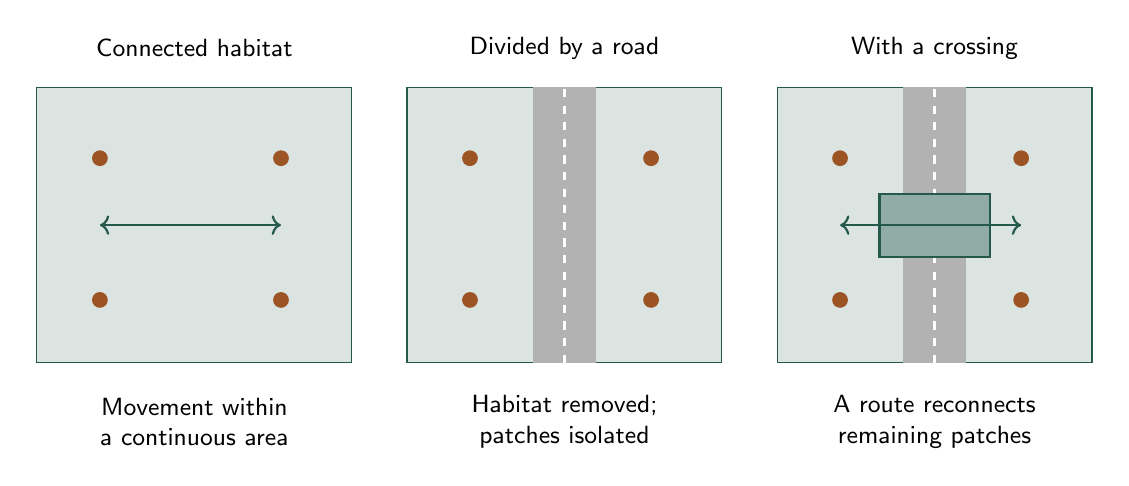
\begin{tikzpicture}[font=\small\sffamily]
\foreach \x/\title in {0/Connected habitat,4.7/Divided by a road,9.4/With a crossing} {
\fill[forest!16] (\x,0) rectangle ++(4,3.5);
\draw[forest] (\x,0) rectangle ++(4,3.5);
\node at (\x+2,4) {\title};
}
\foreach \x in {4.7,9.4} {
\fill[gray!60] (\x+1.6,0) rectangle ++(0.8,3.5);
\draw[white,dashed,thick] (\x+2,0)--++(0,3.5);
}
\fill[forest!50] (10.7,1.35) rectangle (12.1,2.15);
\draw[forest,thick] (10.7,1.35) rectangle (12.1,2.15);
\foreach \x in {0.8,3.1,5.5,7.8,10.2,12.5} {
\fill[orange] (\x,0.8) circle (0.10);
\fill[orange] (\x,2.6) circle (0.10);
}
\draw[<->,thick,forest] (0.8,1.75)--(3.1,1.75);
\draw[<->,thick,forest] (10.2,1.75)--(12.5,1.75);
\node[align=center,text width=4cm] at (2,-0.75) {Movement within\\a continuous area};
\node[align=center,text width=4cm] at (6.7,-0.75) {Habitat removed;\\patches isolated};
\node[align=center,text width=4cm] at (11.4,-0.75) {A route reconnects\\remaining patches};
\end{tikzpicture}\par
\end{center}
\textit{Conceptual landscape, not a measured map.} Dots represent individuals; arrows represent potential movement. Crossings help only if organisms can use them safely.
\subsection*{Four mechanisms}
\begin{enumerate}
\item \textbf{Loss:} development removes feeding and breeding sites. Resource supply and carrying capacity can decrease.
\item \textbf{Isolation:} individuals may struggle to find mates or recolonize a patch. Reduced gene flow can compound the problem over generations.
\item \textbf{Edge effects:} temperature, moisture, predators, and human disturbance may differ near habitat boundaries.
\item \textbf{Connectivity:} a suitable corridor can support migration, mating, and movement toward newly suitable habitat as conditions change.
\end{enumerate}
Protecting large areas and restoring degraded habitat support resource availability. Corridors support movement. A crossing does not eliminate every road hazard or replace all habitat removed by development.
\subsection*{CHIPPO threats can interact}
A road can remove habitat, introduce pollutants, and provide a route for introduced species. Climate change may further reduce the suitability of isolated patches. Identify the interacting mechanisms instead of assigning one label and stopping.
\memorycheck{A corridor increases immigration into one patch. Does that prove the total regional population grew?}
\classsource{Biodiversity Worksheet; Threats to Biodiversity Notes; Ecology 2 framework, page 1.}


\pagechapter{2B\quad Writing a scientific argument}{cer}
\idea{A strong CER answer links a claim to relevant evidence using a biological mechanism.}
\begin{description}[leftmargin=0pt,labelindent=0pt]
\item[Claim] Directly answer the question with a specific, defensible conclusion.
\item[Evidence] Use observations or measurements, including units and meaningful comparisons. Do not invent data.
\item[Reasoning] Explain why the evidence supports the claim using a scientific principle. Address an alternative explanation when relevant.
\end{description}
\subsection*{Worked example with invented practice data}
\textbf{Question:} Does a flower strip appear to support pollinator visits?

In this hypothetical study, three equal-sized plots with flower strips averaged 24 visits per hour; three similar plots without strips averaged 9. Observations used the same duration and comparable weather.

\textbf{Claim.} The results support the idea that flower strips increase pollinator visitation under the conditions tested.

\textbf{Evidence.} Plots with flower strips averaged 24 visits per hour, compared with 9 without strips, a difference of 15 visits per hour.

\textbf{Reasoning.} Flowers provide nectar and pollen, so additional floral resources can attract pollinators. Greater visitation in the plots with flower strips is consistent with that mechanism. More visits do not by themselves prove an increase in pollinator population size or species diversity.

\textbf{Limitation.} Unmeasured plot differences could contribute to the result. Random assignment, repeated sampling, and measuring additional variables would strengthen the inference.
\subsection*{Make each sentence do a job}
\begin{itemize}
\item Name the organism, variable, or resource instead of using a vague pronoun.
\item Replace ``restores balance'' with the mechanism: ``increases prey mortality, reducing grazing pressure.''
\item Use \textbf{because} to connect evidence and mechanism; a repeated claim is not reasoning.
\item Match the strength of the conclusion to the evidence. A correlation can motivate a hypothesis without proving causation.
\end{itemize}
\textbf{Teacher writing emphasis.} Section 1C discourages vague words such as ``thing,'' ``normal,'' and ``balance,'' and asks for care with ``adapt'' and ``healthy.'' Prefer precise processes and measurable outcomes.

\textbf{Adaptation versus immediate response.} Evolutionary adaptation concerns inherited traits across generations. An individual sweating or moving into shade is responding to conditions, not evolving during that event.
\memorycheck{Write a three-sentence CER about habitat fragmentation using the mechanism on the previous page. Label hypothetical evidence as hypothetical.}

\pagechapter{2C\quad Population change and limits}{twoc}
\idea{Population size changes through births, deaths, immigration, and emigration. Resources and conditions affect all four processes.}
A \textbf{population} is a group of organisms of the same species in a defined area. Over a stated interval:
\[
\Delta N=(B+I)-(D+E),\qquad N_{\mathrm{new}}=N_{\mathrm{old}}+\Delta N
\]
$B$ = births, $I$ = immigration (moving in), $D$ = deaths, and $E$ = emigration (moving out). Use counts for the same interval and area.

\textbf{Worked example.} A population starts at 200. There are 40 births, 12 immigrants, 25 deaths, and 7 emigrants:
\[
\Delta N=(40+12)-(25+7)=20,\qquad N_{\mathrm{new}}=220.
\]
A flat population graph does not mean births and deaths stopped; it can mean total gains equal total losses.
\subsection*{Limiting factors}
\par
\begin{tabularx}{\linewidth}{@{}p{0.29\linewidth}Y@{}}\toprule
Type & How to recognize it\\\midrule
Density dependent & Its effect per individual tends to change with crowding. Examples include competition for food or nesting space and transmission of some diseases.\\
Density independent & Its impact is not caused by crowding. A severe freeze, fire, or flood can affect sparse and crowded populations, although actual damage depends on context.\\\bottomrule
\end{tabularx}
\par
\subsection*{Carrying capacity is conditional}
\textbf{Carrying capacity} ($K$) is the population size an environment can support over time with its available resources and conditions. It is specific to the organism, place, and conditions, not a permanent universal number.
\begin{itemize}
\item More usable food or habitat can raise $K$; drought, contamination, and habitat destruction can lower it.
\item As a population grows, resources per individual may decline, lowering birth rates or raising death rates. This can act like negative feedback.
\item Delayed responses, seasons, migration, and changing resources can cause populations to fluctuate around a changing $K$.
\item An extreme event can cause immediate mortality, alter $K$, or both. Overshoot can deplete resources and contribute to a later decline.
\end{itemize}
\memorycheck{A pond dries down to half its area. Explain why fish numbers might decline even if fishing has stopped.}

\pagechapter{2C\quad Reading population graphs}{curves}
\idea{A model simplifies reality. Use its shape to explain a mechanism, then state which conditions the model assumes.}
\begin{center}
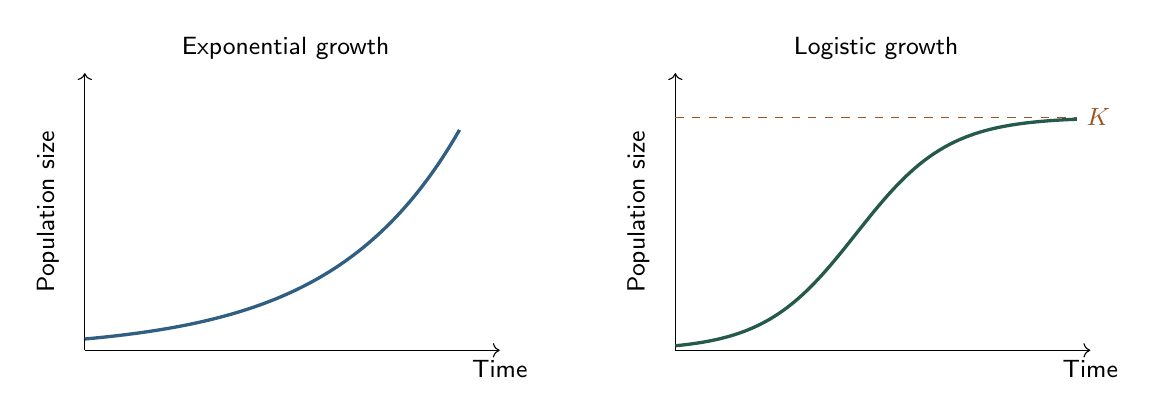
\begin{tikzpicture}[x=0.85cm,y=0.8cm,font=\small\sffamily]
\draw[->] (0,0)--(6.2,0) node[below]{Time};
\draw[->] (0,0)--(0,4.4);
\node[rotate=90] at (-0.55,2.2) {Population size};
\draw[blue,very thick,domain=0:5.6,samples=70] plot (\x,{0.18*exp(0.53*\x)});
\node at (3,4.8) {Exponential growth};
\begin{scope}[xshift=7.5cm]
\draw[->] (0,0)--(6.2,0) node[below]{Time};
\draw[->] (0,0)--(0,4.4);
\node[rotate=90] at (-0.55,2.2) {Population size};
\draw[dashed,orange] (0,3.7)--(6,3.7) node[right]{$K$};
\draw[forest,very thick,domain=0:6,samples=80] plot (\x,{3.7/(1+exp(-1.45*(\x-2.7)))});
\node at (3,4.8) {Logistic growth};
\end{scope}
\end{tikzpicture}\par
\end{center}
\textit{Schematic curves, not observations.} Axes show relative population size and time.

\textbf{Exponential growth} produces a J-shaped curve under sustained positive per-capita growth with resources not yet limiting. A fixed percentage increase means larger populations add more individuals per interval. Growth cannot continue indefinitely in a finite environment.

\textbf{Logistic growth} produces an idealized S-shaped curve. Growth slows as resource limitations increase near $K$. It is useful even though real populations often fluctuate instead of following a perfectly smooth line.
\begin{center}
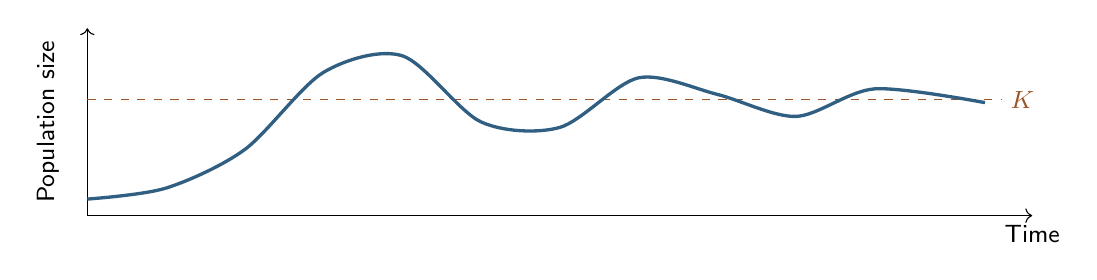
\begin{tikzpicture}[x=1cm,y=0.7cm,font=\small\sffamily]
\draw[->] (0,0)--(12,0) node[below]{Time};
\draw[->] (0,0)--(0,3.4);
\node[rotate=90] at (-0.5,1.7) {Population size};
\draw[dashed,orange] (0,2.1)--(11.6,2.1) node[right]{$K$};
\draw[blue,very thick] plot[smooth] coordinates {(0,0.3)(1,0.5)(2,1.2)(3,2.6)(4,2.9)(5,1.7)(6,1.6)(7,2.5)(8,2.2)(9,1.8)(10,2.3)(11.4,2.05)};
\end{tikzpicture}\par
\end{center}
\textit{Illustrative fluctuation with a reference $K$.} Real $K$ may also change; the horizontal line is an assumption here.
\subsection*{A graph-reading routine}
Read the axes and units; describe where the population rises, falls, or stays similar; compare gains with losses; propose a mechanism; then state what the graph cannot establish. A declining curve alone cannot distinguish increased deaths from increased emigration.
\memorycheck{Near the flat part of a logistic curve, must the birth rate be zero? Explain.}

\pagechapter{2C\quad When carrying capacity changes}{changingk}
\idea{Environmental capacity and actual population size can change at different times. Lower resources do not instantly remove all individuals above a new limit.}
\begin{center}
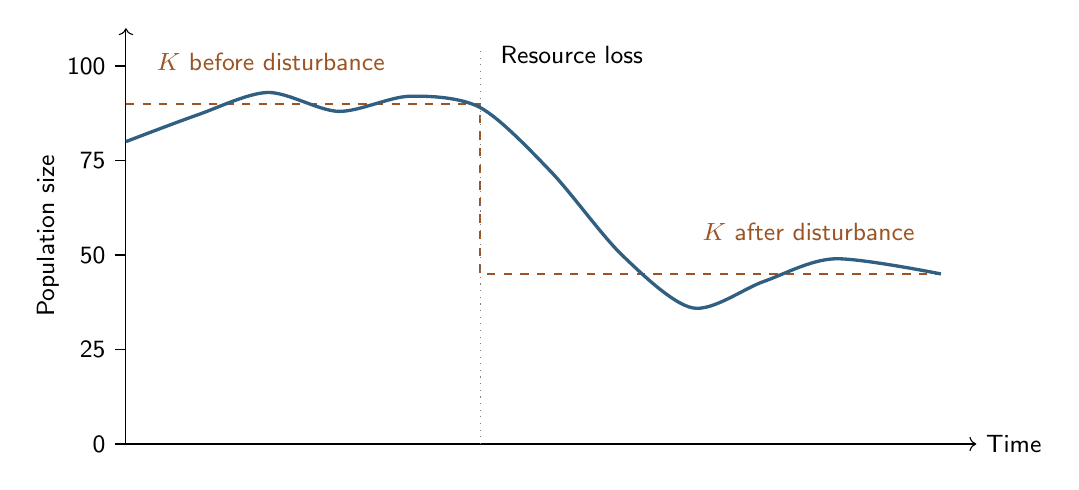
\begin{tikzpicture}[x=0.9cm,y=0.048cm,font=\small\sffamily]
\draw[->] (0,0)--(12,0) node[right]{Time};
\draw[->] (0,0)--(0,110);
\node[rotate=90] at (-1.1,55) {Population size};
\foreach \y in {0,25,50,75,100} {\draw (0,\y)--(-0.15,\y) node[left]{\y};}
\draw[orange,thick,dashed] (0,90)--(5,90)--(5,45)--(11.5,45);
\draw[blue,very thick] plot[smooth] coordinates {(0,80)(1,87)(2,93)(3,88)(4,92)(5,89)(6,72)(7,50)(8,36)(9,43)(10,49)(11.5,45)};
\draw[gray,dotted] (5,0)--(5,105);
\node[anchor=west,text=orange] at (0.3,101) {$K$ before disturbance};
\node[anchor=west,text=orange] at (8,56) {$K$ after disturbance};
\node[anchor=west] at (5.15,103) {Resource loss};
\end{tikzpicture}\par
\end{center}
\textit{Invented illustration.} Orange dashes show $K$; blue shows population size. Values illustrate a pattern, not observations of a particular species.
\subsection*{Interpret the sequence}
Resource loss lowers $K$. The population initially remains above the new capacity, then responds through changes in births, deaths, and movement. Delays and environmental variation can produce later fluctuations.
\begin{center}
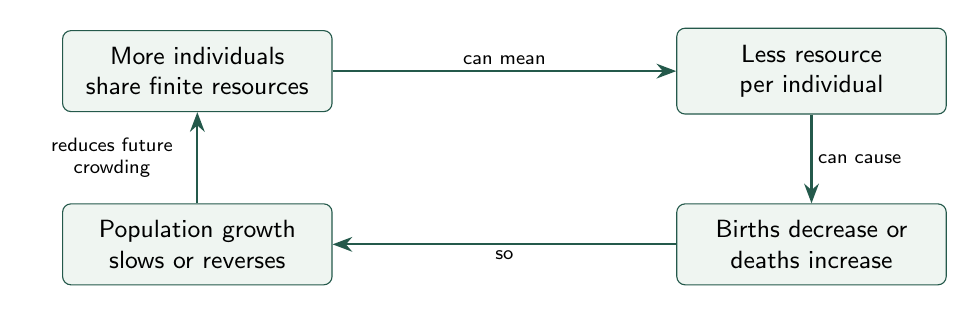
\begin{tikzpicture}[concept/.append style={text width=3cm}]
\node[concept] (n) at (0,0) {More individuals\\share finite resources};
\node[concept] (r) at (7.8,0) {Less resource\\per individual};
\node[concept] (b) at (7.8,-2.2) {Births decrease or\\deaths increase};
\node[concept] (g) at (0,-2.2) {Population growth\\slows or reverses};
\draw[flow] (n)--node[rel,above]{can mean}(r);
\draw[flow] (r)--node[rel,right]{can cause}(b);
\draw[flow] (b)--node[rel,below]{so}(g);
\draw[flow] (g)--node[rel,left,text width=2cm]{reduces future\\crowding}(n);
\end{tikzpicture}\par
\end{center}
\textbf{Size} is a count. \textbf{Density} is individuals per area or volume. \textbf{Dispersion} is their spacing, such as clustered, uniform, or random. \textbf{Demography} includes age structure and patterns of births and deaths. These measurements answer different questions.
\memorycheck{After a wildfire, distinguish immediate mortality from a reduction in the number of organisms the remaining habitat can sustain.}
\classsource{Population Ecology KJ, slides 2--14; Population Ecology Skeleton Notes; Ecology 2 framework, page 2.}


\pagechapter{2C\quad Human resource use}{humans}
\idea{Human demand depends on population, consumption, and technology. Sustainability also depends on regeneration, waste absorption, and who bears the costs.}
\subsection*{Ecological footprint and overshoot}
An \textbf{ecological footprint} estimates demand on biologically productive land and water, including resource provision and carbon dioxide absorption within the accounting framework. \textbf{Biocapacity} describes ecosystems' capacity to regenerate biological resources and absorb the accounted wastes.

\textbf{Earth Overshoot Day} is the estimated date when humanity's cumulative annual demand exceeds what Earth can regenerate that year. Its calculation compares annual biocapacity with annual ecological footprint. An earlier date indicates greater demand relative to regeneration; a later date indicates less. The date is an estimate, changes with demand and biocapacity, and can be revised as data and methods improve. It does not mean all resources physically run out that day, and it is not a direct biodiversity count.
\source{Global Footprint Network, \href{https://overshoot.footprintnetwork.org/about-earth-overshoot-day/}{About Earth Overshoot Day} and \href{https://footprintnetwork.org/our-work/earth-overshoot-day/}{calculation updates}. No particular year's date is needed here.}
\subsection*{Human carrying capacity is not a fixed head count}
Food systems, water availability, energy use, technology, consumption patterns, and environmental damage change how many people can be supported under particular living conditions. Resource extraction can temporarily support high consumption while degrading future productive capacity. ``Renewable'' does not mean available without limits: a forest can regrow, but harvesting faster than regrowth can deplete it.
\subsection*{Environmental justice}
\textbf{Environmental justice} concerns fair treatment and meaningful participation in environmental decisions. Benefits from resource use and burdens from pollution or scarcity are often distributed unequally. Consider who gets clean water, who lives near pollution, who pays for protection, and whose views influence decisions.

\textbf{Example.} Two communities use goods made by the same factory, but only one experiences contaminated local water. Evaluating resource use requires considering the shared benefits, unequal exposure, and access to decision-making, as well as total consumption.
\begin{center}
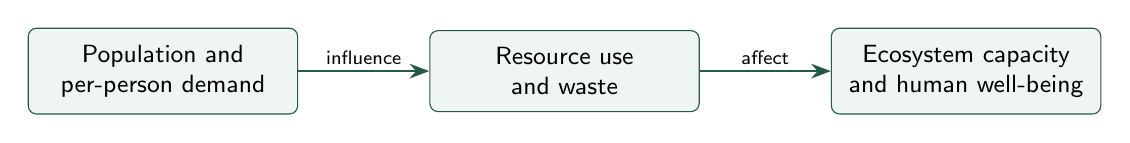
\begin{tikzpicture}[concept/.append style={text width=3cm}]
\node[concept] (a) at (0,0) {Population and\\per-person demand};
\node[concept] (b) at (5.1,0) {Resource use\\and waste};
\node[concept] (c) at (10.2,0) {Ecosystem capacity\\and human well-being};
\draw[flow] (a)--node[rel,above]{influence}(b);
\draw[flow] (b)--node[rel,above]{affect}(c);
\end{tikzpicture}\par
\end{center}
\memorycheck{Explain how reducing wasted food could reduce demand without reducing the number of people fed.}

\pagechapter{2C\quad Resource demand and environmental justice}{resources}
\idea{Human carrying capacity depends on how resources are used and shared, not just on the number of people.}
\subsection*{Understand the Overshoot Day comparison}
Earth Overshoot Day compares annual ecological demand with annual biological regeneration. In the accounting framework:
\[
\text{day of year}\approx
\frac{\text{annual biocapacity}}{\text{annual ecological footprint}}
\times\text{days in the year}.
\]
\textbf{Hypothetical example.} If annual demand is twice annual biocapacity, the ratio is $1/2$. In a 365-day year, the corresponding date is around day 183. Reducing demand to $1.5$ times capacity moves the comparison to about day 243. These are illustrations, not actual annual dates.
\subsection*{What continued overshoot means}
The population slides describe using resources accumulated in the past, reducing resources available to other organisms and people in the present, and limiting future options. Examples include drawing down slowly replenished groundwater, removing old forests, and using fossil fuels. These examples explain resource pressure; Overshoot Day does not directly measure every resource stock.

\textbf{Biocapacity} is productive capacity, while \textbf{ecological footprint} measures demand in a specified accounting system. A date change can reflect demand, biocapacity, or revised estimates. It cannot by itself establish a particular number of species lost.
\subsection*{Quality of life and fairness}
A higher quality of life does not always require proportionally more resources. Less food waste, efficient buildings, and effective public services can deliver benefits with less input. Technology can improve efficiency, but environmental damage and rebound in consumption can offset gains.

Environmental justice asks who receives the benefits, who experiences pollution or scarcity, and who participates in decisions. A strategy that lowers total consumption can still distribute costs unfairly. Evaluate the ecological mechanism and the distribution of consequences.
\subsection*{Explain a solution with a causal chain}
Reducing food waste can reduce demand for crops, land, water, and energy while maintaining nutrition. Habitat restoration can improve productive capacity and biodiversity. Neither example guarantees a particular global date shift; the outcome depends on scale and other changes.
\memorycheck{Explain why increasing resource extraction now can support short-term consumption while lowering future carrying capacity.}
\classsource{Population Ecology KJ, slides 17--19; Ecology 2 framework, page 2. Formula: \href{https://overshoot.footprintnetwork.org/about-earth-overshoot-day/}{Global Footprint Network}.}


\pagechapter{Vocabulary for precise explanations}{vocab}
The biological terms are defined in their topic sections. These academic words help you express the relationships the teacher asks about.
\par
\begin{tabularx}{\linewidth}{@{}p{0.32\linewidth}Y@{}}\toprule
Words & Meaning in a biology explanation\\\midrule
Assess; assessment & Evaluate understanding or performance against criteria.\\
Commitment; effective & Sustained effort; successful in achieving an intended result.\\
Condition; criteria & A circumstance affecting a system; standards used to judge a claim or classify something.\\
Stable; constant; range & Stable permits bounded variation; constant is unchanging; range is the span of values.\\
Dynamic; equilibrium & Dynamic means changing or involving ongoing processes. Equilibrium describes opposing processes with no net change; homeostasis generally requires ongoing regulation.\\
Mechanism; model & A process explaining how an effect occurs; a simplified representation used to explain or predict.\\
Reinforce & Strengthen a response or change, as in positive feedback.\\
Affect; effect & Affect is usually a verb meaning influence; effect is usually a noun meaning result.\\
Convert; transfer; store & Change form; move between locations or organisms; retain for later use. Energy is transformed or transferred, not created by organisms.\\
Obtain; release; generate & Acquire; let out; produce. Say organisms generate ATP or heat, not that they create energy from nothing.\\
Cycle; process; interact & Move through repeated transfers; a sequence of events; influence one another.\\
Efficient & Producing a given output with less input or waste; specify which input and output.\\
Complex; context; diverse & Having many interacting parts; relevant circumstances; varied in composition.\\
Collapse; resilient & Severe loss of structure or function; able to retain or recover function after disturbance.\\
Resources & Materials, energy sources, or conditions organisms use to survive and reproduce.\\\bottomrule
\end{tabularx}
\par
\memorycheck{Use ``transfer,'' ``convert,'' and ``release'' in three separate accurate sentences about energy.}

\pagechapter{Vocabulary for ecological change}{vocabtwo}
\par
\begin{tabularx}{\linewidth}{@{}p{0.32\linewidth}Y@{}}\toprule
Words & Meaning in a biology explanation\\\midrule
Consumption; exploitation & Use of resources; use or harvest of organisms or resources. Overexploitation exceeds replacement capacity.\\
Destruction; disruption & Removal or severe damage; interference with a process or relationship.\\
Impact; threat & An effect; a potential cause of harm. State the affected organism or process.\\
Migration & Movement between locations, often seasonal; immigration and emigration specify movement relative to a defined population.\\
Prevention; restoration & Avoiding a problem; helping a damaged ecosystem recover structure or functions.\\
Capacity; finite & The amount that can be supported or held; limited in quantity.\\
Decline; fluctuate & Decrease; vary upward and downward over time.\\
Exacerbate; exceed & Make a problem worse; go beyond a limit.\\
Factor; outcome & Something contributing to a result; the result itself.\\
Indefinitely; limit & Without an end; a constraint or boundary. Exponential growth cannot continue indefinitely with finite resources.\\
Replenish & Replace resources as they are used, through regeneration or other supply.\\\bottomrule
\end{tabularx}
\par
\subsection*{Six statements to be able to explain without notes}
\begin{enumerate}
\item An observation and an inference serve different roles in a scientific explanation.
\item Negative feedback opposes a change; homeostasis allows bounded variation.
\item Producers and consumers both use cellular respiration, while producers supply new organic matter to food webs.
\item Energy dissipates as heat; atoms return through matter cycles.
\item Biodiversity can support resilience, but particular species and disturbance conditions matter.
\item Population growth reflects gains, losses, and limits; carrying capacity can change.
\end{enumerate}
\subsection*{Connect rather than memorize}
Complete this sentence with a mechanism: ``A drought can change carrying capacity because \ldots'' Then connect that mechanism to producer growth, herbivore food supply, and biodiversity. This single chain uses ideas from 1C, 2A, and 2C.

\pagechapter{Review questions\quad Foundations}{practiceone}
These are new practice questions, not copied exam questions. Answer on separate paper before reading the explanations.
\begin{enumerate}
\item \textbf{1A.} A student records 18 snails in a shaded plot and 6 in a sunny plot, then says shade causes more snails to survive. Identify one observation and one inference. Give a possible confounding factor.
\item \textbf{1A.} Write an inductive conclusion and a deductive prediction about the effect of moisture on seedling growth. Explain the difference.
\item \textbf{1B.} Body temperature falls; shivering starts; temperature rises toward its regulated range. Identify the feedback type and explain why the word ``negative'' applies.
\item \textbf{1B.} A student says a plant cannot be alive because it does not walk and cannot reproduce yet. Explain why those facts do not establish the conclusion.
\item \textbf{1C.} Complete the comparison: photosynthesis takes in which gas and releases which gas? Aerobic cellular respiration does the reverse for which gases? Explain whether a plant respires.
\item \textbf{1C.} In the chain grass $\to$ rabbit $\to$ fox, describe the arrow direction. Explain why a fox depends on producers even though it does not eat grass.
\item \textbf{1C.} Producers supply 20,000 energy units per area per year. Assuming 10\% transfer at each step, calculate energy reaching secondary consumers. Explain where energy not transferred to that level can go.
\item \textbf{1C.} A decomposer community declines sharply. Predict one immediate change in dead material and one later effect on producers. State the connecting mechanism.
\item \textbf{1C.} Explain two reasons why a top predator can be vulnerable when habitat is reduced. Connect each reason to its food web or ecological pyramid.
\end{enumerate}
\vfill
\textbf{Self-check.} Could someone follow the cause-and-effect steps in your answer without guessing what ``it'' or ``balance'' means?

\pagechapter{Review questions\quad Ecological change}{practicetwo}
\begin{enumerate}[start=10]
\item \textbf{2A.} Two fields each have five pollinator species. In one, nearly all visits come from one species; in the other, visits are more evenly shared. What feature differs? Why might it matter after disturbance?
\item \textbf{2A.} Give one ecosystem service used by humans and trace the ecological process providing it. Name its service category.
\item \textbf{2B.} Expand CHIPPO. Choose two threats and give a conservation response matched to each mechanism.
\item \textbf{2B.} A road separates a forest into two patches. Explain how a wildlife corridor may help and why habitat protection is still needed.
\item \textbf{2B.} In a hypothetical experiment, 8 of 10 native seedlings survive without an introduced herbivore, compared with 3 of 10 with it. Write a CER about the herbivore's effect. State one limitation.
\item \textbf{2C.} A population starts at 500. In a year there are 90 births, 35 deaths, 20 immigrants, and 45 emigrants. Calculate its new size.
\item \textbf{2C.} Contrast exponential and logistic growth. Explain why a smooth logistic curve is useful even though a real population fluctuates.
\item \textbf{2C.} A drought lowers food supply while a population is above its former carrying capacity. Predict likely consequences and identify what can happen to $K$.
\item \textbf{2C.} Explain what an earlier Earth Overshoot Day indicates. Does that date alone measure the number of species lost? Explain.
\item \textbf{2C.} A factory supplies products nationwide but pollutes one community's water. Explain how environmental justice relates to the situation.
\item \textbf{Across sections.} Construct a five-node knowledge graph beginning with habitat loss and ending with an effect on people. Label every arrow and state one condition that could change your prediction.
\end{enumerate}
\vfill
\textbf{For diagrams.} State whether your arrows show feeding, movement of matter, energy transfer, or cause and effect. Do not silently change arrow meanings.

\pagechapter{Diagram review\quad Applying the class material}{diagrampractice}
These are original review questions based on the supplied class tasks. Draw and explain your answers before checking the answer guide.
\begin{enumerate}
\item \textbf{Cell and virus.} Label a cell membrane, genome, and cellular machinery. Draw a virus beside it and apply the life checklist.
\item \textbf{Feedback.} Draw both branches of temperature regulation. Label condition, response, resulting change, and reduced corrective action.
\item \textbf{Gas and energy.} Draw sunlight, a plant, a rabbit, and aerobic decomposers. Add heat arrows for all living groups and the correct gas arrows to the surroundings.
\item \textbf{Lab.} In invented data, 0.50 L of water warms by $3.0^\circ$C. Estimate heat gained in Calories. Explain the purpose of the no-hand control.
\item \textbf{Biodiversity.} Illustrate variation within one species and variation among species. Explain why the pictures represent different levels.
\item \textbf{Corridor.} Draw a habitat divided by a road and a crossing. Explain effects on movement, gene flow, and habitat amount.
\item \textbf{Changing capacity.} Lower $K$ after a disturbance and draw a delayed population response. Explain the mechanisms.
\item \textbf{CER.} Use actual lab data if available to write a temperature-comparison claim. Separate measured warming from the proposed metabolic explanation.
\item \textbf{Life.} Compare a dormant seed, a fire, and a sterile animal using at least three characteristics.
\item \textbf{Energy.} Explain how digestion, cellular respiration, ATP, and homeostasis are related without saying that matter becomes energy.
\item \textbf{Resources.} If hypothetical demand is 1.25 times annual biocapacity, estimate the corresponding day in a 365-day year. Explain what that comparison does and does not measure.
\item \textbf{Conservation.} A habitat corridor increases movement, but pollution remains. Explain why population recovery is not guaranteed.
\end{enumerate}
\textbf{Diagram checklist.} Label axes and units. Distinguish real data from schematics. Give each arrow a clear meaning and each causal connection a mechanism.


\pagechapter{Answer explanations\quad Foundations}{answersone}
\begin{enumerate}
\item The counts (18 and 6) are observations. The claim about shade causing survival is an inference. Moisture, food, sampling area, or detection could differ. Counts alone do not measure survival rates.
\item Induction: repeated observations suggest that seedlings with adequate moisture grow more. Deduction: if water limits growth, otherwise comparable dry seedlings should grow more when supplied with water. Induction develops a broader idea; deduction predicts a specific outcome from it.
\item Negative feedback: the initial decrease triggers a response that increases temperature, opposing the initial change. The response is not ``negative'' because it is harmful.
\item Locomotion is not a universal criterion for life. A young plant can be cellular, metabolically active, regulated, and developing even before reproductive maturity. Consider the full set of characteristics.
\item Oxygen-producing photosynthesis takes in carbon dioxide and releases oxygen. Aerobic respiration consumes oxygen and releases carbon dioxide. Plants carry out respiration to supply energy for cellular work; photosynthesis does not replace that need.
\item Arrows point from food to consumer, showing transfer of organic matter and chemical energy. Grass supplies the rabbit's food; the fox receives some of that matter and energy by eating the rabbit.
\item $20{,}000(0.10)^2=200$ units per area per year. Energy can be released as metabolic heat or remain in material not passed to the next consumer, including waste and uneaten parts that can support decomposers. Energy is not destroyed.
\item Dead material tends to accumulate. Slower decomposition reduces the return of available nutrients, which can later limit producer growth. Timing depends on existing nutrients and other recycling pathways.
\item Lower energy availability supports fewer individuals at high trophic levels, so additional losses can strongly affect a small population. A predator also needs enough connected habitat and prey production; habitat reduction can shrink the supporting prey base or hunting area. These are tendencies, not guarantees for every species.
\end{enumerate}
\subsection*{Answers to the short memory prompts}
A strong answer names the original change, the mechanism, and the result. For food-web questions, distinguish transfer of atoms from transfer and dissipation of energy. For the graph on page \pageref{web}, rabbits offer the hawk an alternative food source, but their abundance may not be sufficient to replace frogs.

\pagechapter{Answer explanations\quad Ecological change}{answerstwo}
\begin{enumerate}[start=10,itemsep=5pt]
\item Species richness is equal; relative contribution to visits differs. Visit counts alone do not establish the abundance of each species. More evenly distributed activity may reduce dependence on one species. Resilience still depends on how each species responds and whether others can compensate.
\item Example: pollinators transfer pollen, helping crops reproduce and produce fruits or seeds used as food. Pollination is commonly a regulating service; harvested food is provisioning. Explain the process even when a category is not required.
\item Climate change, habitat loss, invasive species, pollution, population, overexploitation. Examples: habitat protection addresses loss; harvest limits address removal faster than reproduction; pollution control reduces exposure.
\item A corridor can permit movement, mating, and recolonization, reducing isolation. It cannot replace all lost feeding or breeding habitat. Design, safety, and the species' behavior affect its usefulness.
\item Claim: the herbivore reduced seedling survival in the trial. Evidence: survival was 3/10 with it versus 8/10 without it. Reasoning: feeding damage can remove tissue needed for photosynthesis or growth. A small sample and unmeasured differences limit inference; introduction alone does not establish invasive status.
\item $\Delta N=90+20-35-45=30$; the new population is $530$.
\item Exponential growth assumes sustained positive per-capita growth without effective resource limitation. Logistic growth incorporates slowing near $K$. Its idealized pattern helps explain density-related limits even when real resources and population sizes vary.
\item Reduced food can lower $K$. Births may decline, deaths or emigration may rise, and overshoot may further deplete resources. Exact timing and magnitude require data.
\item Demand exceeds annual regeneration earlier in the year. This is a resource-accounting indicator, not a measurement of species loss. Resource pressure can harm biodiversity, but biodiversity change needs separate evidence.
\item Benefits are widespread while pollution burdens are concentrated. Fair access to clean water, protection, and meaningful participation by affected residents are environmental-justice concerns.
\item One valid graph: habitat loss $\to$ fewer flowering plants $\to$ less pollinator food $\to$ fewer pollinator visits $\to$ lower crop pollination. Each arrow means ``can cause.'' Other food sources or managed pollination could change the prediction; lower visits do not automatically prove population decline.
\end{enumerate}

\pagechapter{Diagram review\quad Answer guide}{diagramanswers}
\begin{enumerate}[itemsep=5pt]
\item Cells have membranes and metabolic machinery. Viruses contain a genome and coat but require a host cell to assemble new particles. Shared genetic information alone does not establish cellular life.
\item Warming triggers cooling; cooling reduces the need for further cooling. Falling temperature triggers warming; recovery reduces warming responses. Both oppose the initiating change.
\item Light reaches the plant. Organic molecules move along feeding and decomposition pathways. Every living group releases heat. Photosynthesis takes in carbon dioxide and releases oxygen; aerobic respiration reverses these gas directions. Plants need both sets of arrows.
\item $Q=0.50\times3.0=1.5$ Cal, or 1.5 kcal. The control measures changes possible without a hand. Water heating does not capture all energy used by the body.
\item Allelic differences within a species illustrate genetic diversity; different species illustrate species diversity. Individual counts alone establish neither.
\item A usable crossing can support movement, mating, and recolonization without restoring all removed habitat. Movement into a patch may be redistribution rather than regional growth.
\item Actual numbers can initially exceed the new $K$. Reduced births, increased deaths, or emigration can follow. Exact rates require evidence.
\item Cite actual temperatures and elapsed time. Muscle work uses ATP, metabolism supplies usable energy, and heat transfers to the water. Mixing, hand differences, and starting conditions also affect the measured change.
\item The seed has living cells and genetic information despite dormancy. Fire lacks cells and a biological inheritance system. A sterile animal has cellular organization and metabolism despite reproductive inability.
\item Digestion prepares molecules for absorption. Respiration transfers fuel energy to ATP; ATP supports work needed for homeostasis. Atoms are rearranged, and heat is released.
\item $365/1.25=292$: approximately day 292. This illustrates demand relative to regeneration, not the day all resources physically disappear.
\item Pollution can still reduce survival or reproduction. Connectivity addresses one mechanism; recovery also depends on habitat quality and other limiting factors.
\end{enumerate}
\classsource{Original questions and answers based on the class materials cited in the corresponding chapters.}

\pagechapter{Using the supplied practice key carefully}{keynotes}
The supplied file is titled \textit{StudyBio's Practice Ecology Quiz}. It contains 15 multiple-choice questions and one free-response item, with highlighted answers and comments. It is useful practice, but several statements require interpretation or clarification. Keep the original key intact.
\par
\begin{tabularx}{\linewidth}{@{}p{0.13\linewidth}Y@{}}\toprule
Item & What to learn accurately\\\midrule
Q1 & The arrows depict negative feedback. The key also marks the depiction as incorrect, apparently because the labels describe a fixed temperature. That rationale is inferred, not stated. Homeostasis regulates a range; a simplified diagram is not automatically invalid.\\
Q3 & The key selects ``none of the above'' and names the Sun in a note. Sunlight supports most ecosystems, but chemical energy can support chemosynthetic food webs. ``All life'' is too broad.\\
Q5 & Photosynthesis and chemosynthesis can support production of organic molecules. Chemosynthesis uses chemical energy; lack of oxygen is not its defining feature. Cellular respiration is also used by many producers.\\
Q7 & The key rejects the listed combinations. Removing a consumer does not establish immediate changes in every other group. Follow the actual web and distinguish short-term from delayed effects.\\
Q13 & The key selects ``none'' for corridors directly alleviating habitat loss. The likely intended distinction is loss versus fragmentation. Corridors address connectivity and may also restore habitat; the question's wording does not support a universal rejection of corridors.\\
Q14 & The key calls a smooth logistic curve unrealistic. Treat the curve as an idealized model: useful for explaining limits, but not an exact trace of most field populations.\\
Q15 & The key links an earlier Overshoot Day to biodiversity loss. The direct meaning is greater demand relative to annual regeneration. Species loss cannot be established from the date alone.\\\bottomrule
\end{tabularx}
\par
\textbf{Class requirements clarified.} Although the practice key calls some topics class-dependent, the supplied Biodiversity Worksheet explicitly asks for all four ecosystem-service categories and wildlife corridors. Study both.

\textbf{Review strategy.} Attempt the blank quiz first, then compare explanations with the key. When an answer depends on wording, distinguish the intended classroom concept from a statement that is universally true. Ask the teacher about the highlighted ambiguities before using them as exam rules.

\pagechapter{Sources and coverage}{sources}
\subsection*{Class and practice materials}
\begin{itemize}
\item \textit{Ecology Unit Guide (KJ).docx}: learning targets 1A, 1B, 1C, 2A, 2B, and 2C; vocabulary and study-question scope. The guide's listed textbook sections are retained below. The textbook is identified by Shawn's parent as \textit{California Miller \& Levine Biology Student}; the edition and textbook pages have not yet been supplied.
\item \textit{A\_EcologyPracticeQuiz\_KEY.pdf}: StudyBio practice quiz, four pages. Used to identify question styles, CHIPPO wording, extensions, and key ambiguities. This book does not reproduce the quiz.
\item \textit{A\_EcologyPracticeQuiz\_BLANK.pdf}: companion practice paper available in the project for independent attempts.
\end{itemize}
This revision incorporates text from all 26 supplied source files, including eight slide decks, class worksheets, skeleton notes, CER materials, the energy-flow lab, and the Ecology 2 framework. The two copies of the Ecology 2 framework are identical. Class-connection notes identify the relevant sources throughout. Original explanations, diagrams, synthetic data, and new questions supplement the supplied materials; they are not teacher-issued answers. Linked videos and textbook pages were not supplied or reviewed.
\par
\begin{tabularx}{\linewidth}{@{}l l Y@{}}\toprule
Target & Guide textbook reference & Book focus\\\midrule
1A & Not listed & Evidence, reasoning, and deliberate practice\\
1B & 1.3 & Life, metabolism, feedback, and investigation\\
1C & 3.1, 4.1, 4.2, 6.1 & Ecosystems, food webs, energy and matter\\
2A & 6.3 & Biodiversity, resilience, ecosystem services\\
2B & 7.2 & Human threats, conservation, and CER\\
2C & 5.1, 5.2, 5.3 & Population change, limits, and resource use\\\bottomrule
\end{tabularx}
\par
\subsection*{Supplemental verification and further reading}
\begin{itemize}
\item OpenStax Biology 2e: \href{https://openstax.org/books/biology-2e/pages/1-2-themes-and-concepts-of-biology}{Themes and Concepts of Biology}; \href{https://openstax.org/books/biology-2e/pages/33-3-homeostasis}{Homeostasis}.
\item OpenStax Biology 2e: \href{https://openstax.org/books/biology-2e/pages/46-2-energy-flow-through-ecosystems}{Energy Flow through Ecosystems}, for chemosynthesis and ecological-pyramid qualifications.
\item OpenStax Biology 2e: \href{https://openstax.org/books/biology-2e/pages/45-4-population-dynamics-and-regulation}{Population Dynamics and Regulation}, for model limitations.
\item USDA Forest Service: \href{https://research.fs.usda.gov/treesearch/52660}{Biological corridors and connectivity}, for the distinction between habitat amount and connectivity.
\item Convention on Biological Diversity: \href{https://www.cbd.int/invasive}{Invasive Alien Species}.
\item Global Footprint Network: \href{https://overshoot.footprintnetwork.org/about-earth-overshoot-day/}{About Earth Overshoot Day}; \href{https://footprintnetwork.org/our-work/earth-overshoot-day/}{Earth Overshoot Day and revisions}.
\end{itemize}
\textbf{Next revision.} Add textbook pages and teacher feedback, and update practice around Shawn's missed questions. Material after 2C remains outside this edition.
\end{document}
